\documentclass[9pt]{beamer}

\usepackage{appendixnumberbeamer}
\usepackage{booktabs}
\usepackage[scale=2]{ccicons}
\usepackage{pgfplots}
\usepackage{tikz}
\usepackage{graphics}

\usepgfplotslibrary{dateplot}
\pdfstringdefDisableCommands{\def\translate#1{#1}}
\geometry{paperwidth=140mm, paperheight=105mm}
\usetheme{metropolis}
\bibliographystyle{abbrv}
\setbeamertemplate{frame footer}{Data Analysis And Experimental Characterization For Mechatronic And Robotic Systems}

\usetikzlibrary{shapes, arrows}
\tikzstyle{startstop} = [rectangle, rounded corners, minimum width=2cm, minimum height=1cm, text centered, draw=black, fill=red!30]
\tikzstyle{io} = [trapezium, trapezium stretches=true, trapezium left angle=70, trapezium right angle=110, minimum width=2cm, minimum height=1cm, text centered, draw=black, fill=blue!30]
\tikzstyle{process} = [rectangle, minimum width=2cm, minimum height=1cm, text centered, text width=2cm, draw=black, fill=orange!30]
\tikzstyle{decision} = [diamond, minimum width=2cm, minimum height=1cm, text centered, draw=black, fill=green!30]
\tikzstyle{arrow} = [thick,->,>=stealth]

\title{Structural Health Monitoring (SHM) as a multivariate outlier detection problem}
\subtitle{Tie-rods case study}
\date{Date to be defined}
\author{Tommaso Bocchietti}
\institute{Politecnico di Milano}
\titlegraphic{\hfill
\includegraphics[height=1.5cm]{pdf/Polimi_logo_header.pdf}}

\begin{document}

\maketitle

\begin{frame}{Agenda}

    \begin{columns}[c, onlytextwidth]

        \begin{column}{0.5\textwidth}

            \setbeamertemplate{section in toc}[sections numbered]
            \tableofcontents

        \end{column}

        \begin{column}{0.5\textwidth}

            \begin{figure}[H]
                \centering
                % https://www.architectmagazine.com/technology/iron-found-to-be-an-essential-element-in-gothic-architecture_o
                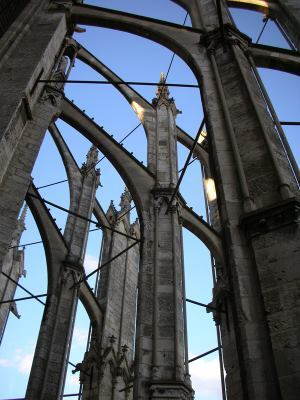
\includegraphics[width=0.8\textwidth]{img/tie-rods-cathedral.jpeg}
                \caption{Steel tie-rods connect the buttresses of the Cathedral of Saint Peter of Beauvais in France.}
            \end{figure}

        \end{column}

    \end{columns}

\end{frame}


\section{Motivations}

\begin{frame}{$\mathrm{CO_2}$ Emission by Sector}

    Transportation sector is the second-largest contributor to $\mathrm{CO_2}$ emission.

    \vspace{9pt}

    \begin{figure}
        \centering
        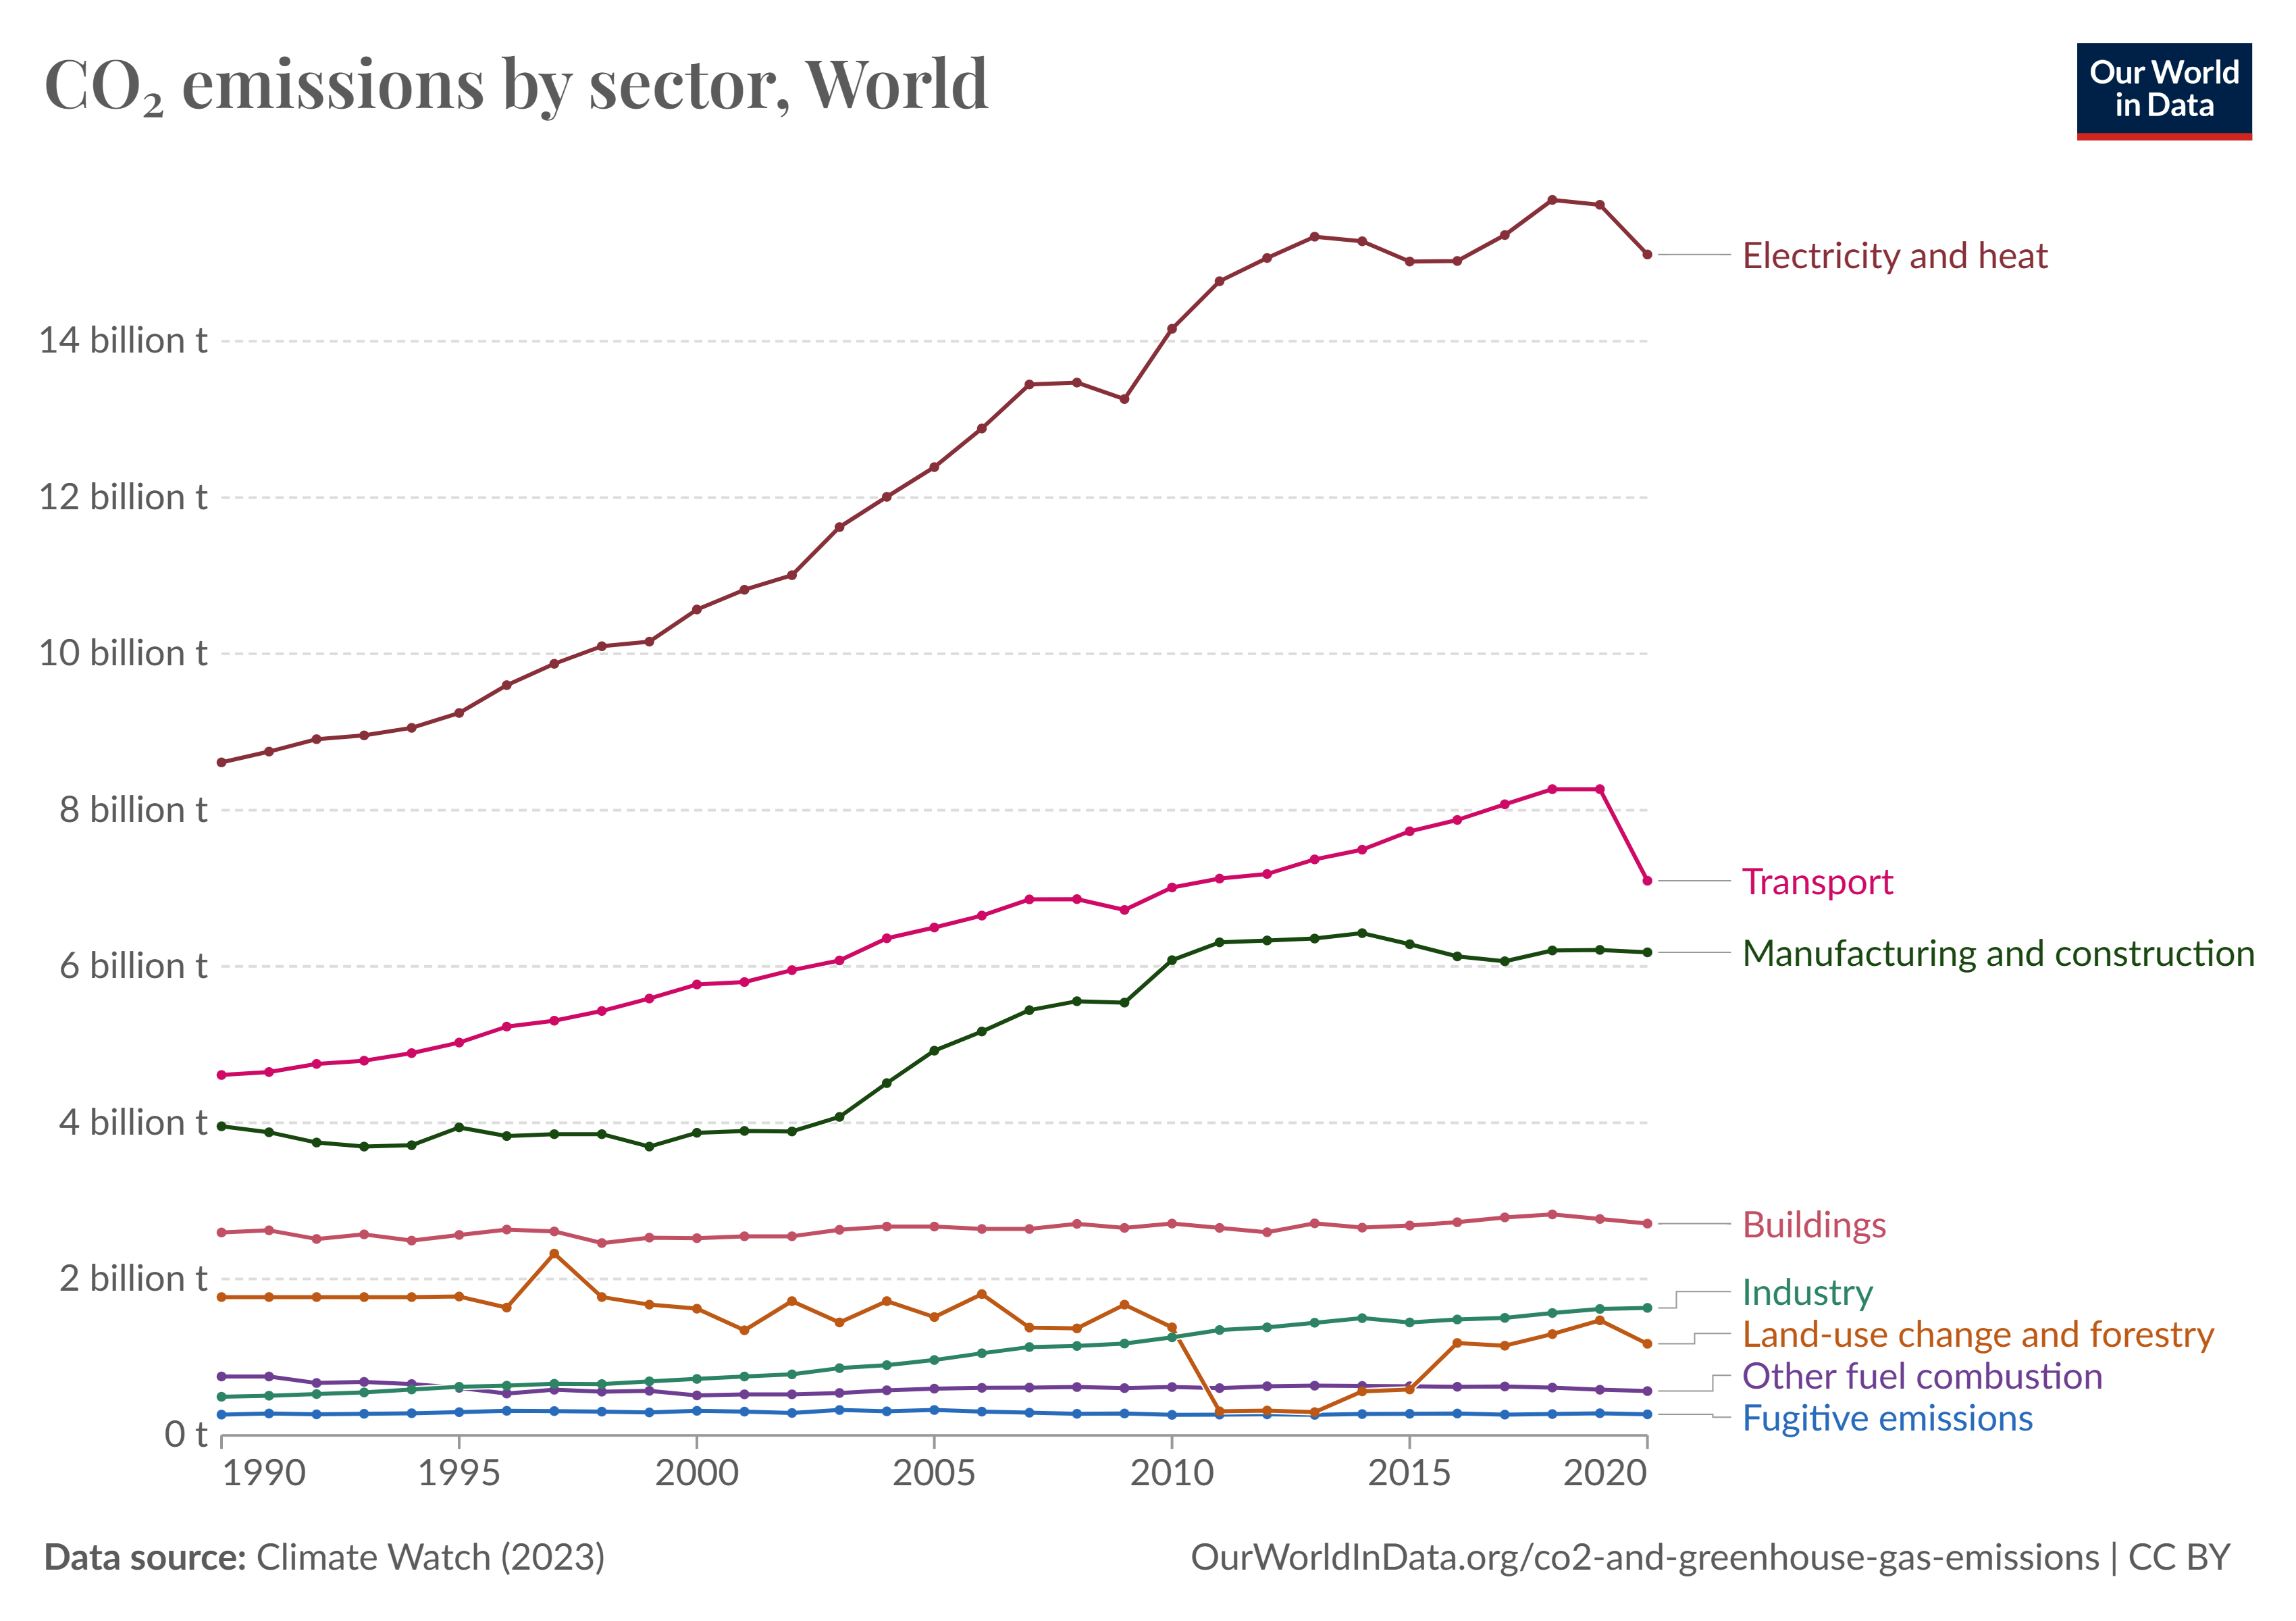
\includegraphics[width=0.8\textwidth]{img/co-emissions-by-sector.png}
        % \caption{$\mathrm{CO_2}$ Emission by sector}
    \end{figure}

\end{frame}



\begin{frame}{Alternative to traditional Fossil Fuel}

    Transportation sector has been looking for alternative fuels to reduce $\mathrm{CO_2}$ emission.

    \begin{itemize}
        \item \textbf{Electricity:} requires a large infrastructure to support the global demand
        \item \textbf{Methane:} worse than $\mathrm{CO_2}$ in terms of greenhouse effect (short-term)
        \item \textbf{Hydrogen:} difficult to store and transport
    \end{itemize}

\end{frame}



\begin{frame}{Ammonia as a Fuel}

    Researchers started looking at Ammonia as a potential alternative fuel.

    \vspace{9pt}

    \begin{columns}[c, onlytextwidth]

        \begin{column}{0.45\textwidth}

            \begin{figure}[H]
                \centering

                \LARGE
                \setchemfig{atom sep=5em, bond offset=5pt}
                \chemfig{\charge{90=\:}{N}(-[:210]H)(<[:290]H)(<:[:-15]H)}
                \normalsize

                \caption{Ammonia molecule ($\mathrm{NH_3}$)}

            \end{figure}

        \end{column}

        \begin{column}{0.55\textwidth}

            Advantages of Ammonia:

            \begin{itemize}
                \item No carbon content (zero $\mathrm{CO_2}$ emission)
                \item Long history of use in the chemical industry
                \item Possible use as hydrogen carrier
            \end{itemize}

        \end{column}

    \end{columns}

\end{frame}



\begin{frame}{Ammonia as a Fuel}

    \begin{columns}[c, onlytextwidth]

        \begin{column}{0.33\textwidth}

            \begin{figure}[H]
                \centering
                
\includegraphics[width=0.5\textwidth]{pdf/nfpa-diesel.pdf}
            \end{figure}

        \end{column}

        \begin{column}{0.33\textwidth}

            \begin{figure}[H]
                \centering
                
\includegraphics[width=0.5\textwidth]{pdf/nfpa-gasoline.pdf}
            \end{figure}

        \end{column}

        \begin{column}{0.33\textwidth}

            \begin{figure}[H]
                \centering
                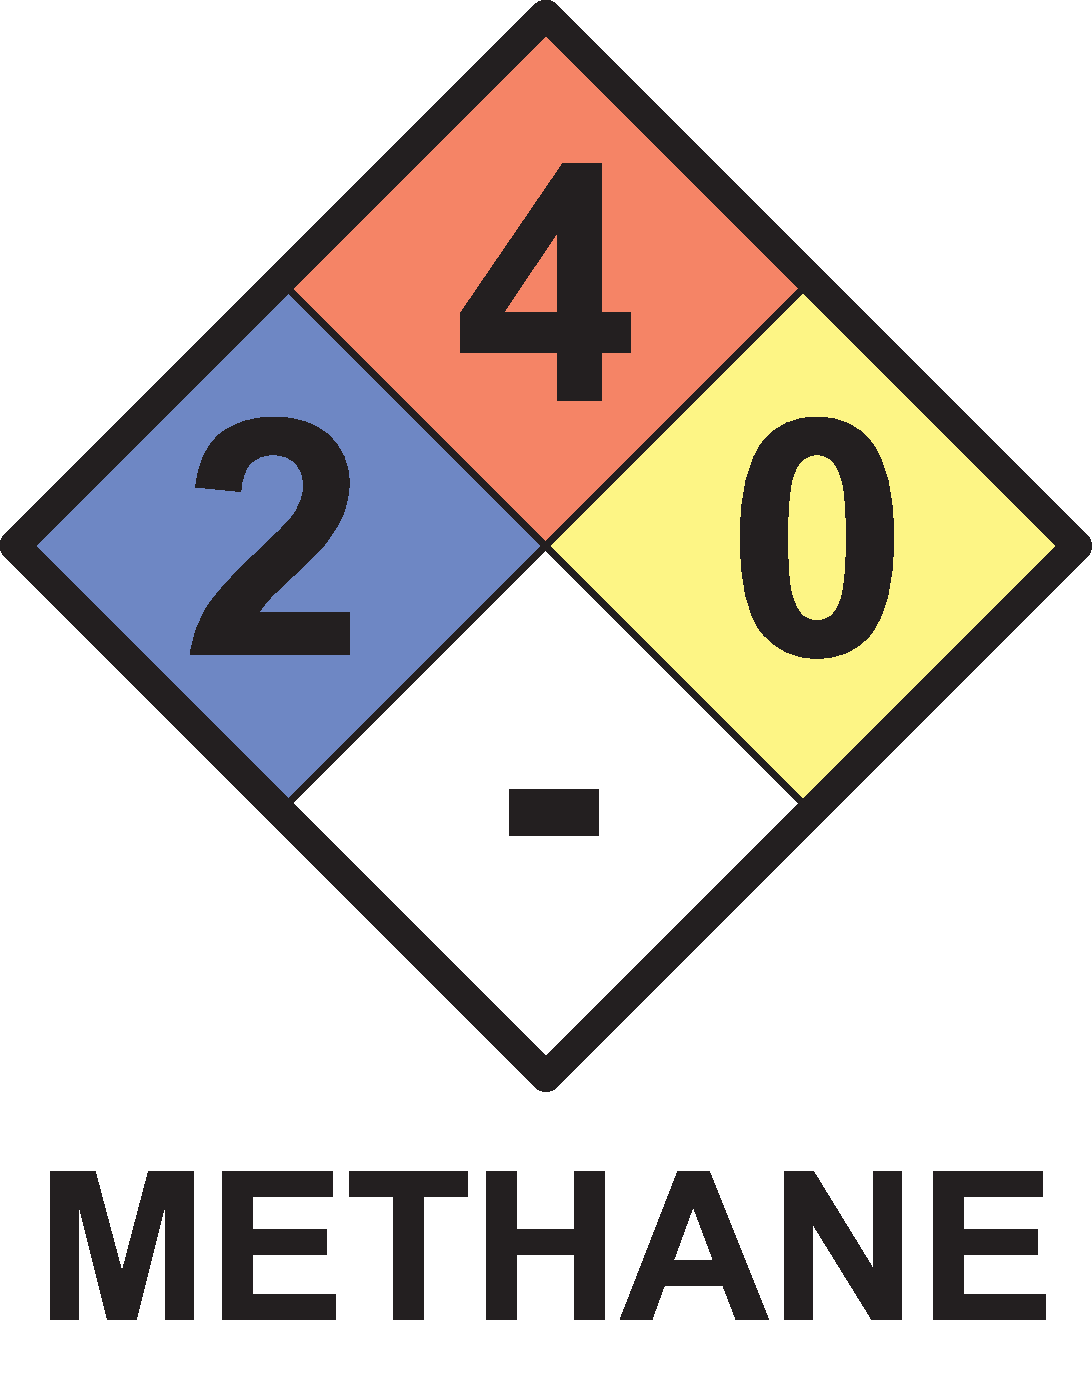
\includegraphics[width=0.5\textwidth]{pdf/nfpa-methane.pdf}
            \end{figure}

        \end{column}

    \end{columns}

    \begin{columns}[c, onlytextwidth]

        \begin{column}{0.4\textwidth}

            \begin{figure}[H]
                \centering
                
\includegraphics[width=0.5\textwidth]{pdf/nfpa-ammonia.pdf}
            \end{figure}

        \end{column}

        \begin{column}{0.6\textwidth}

            Disadvantages of Ammonia (also based on NFPAs\footnotemark[1]):

            \begin{itemize}
                \item Least flammable source, which also suggest \textbf{slow flame speed}
                \item Its combustion might produce \textbf{high $\mathrm{NO_x}$ emissions} if not properly controlled
                      % \item High ignition temperature
                      % Low flame velocity
                      % Slow chemical kinetics
            \end{itemize}

        \end{column}

    \end{columns}

    \footnotetext[1]{National Fire Protection Association 704: Standard System for the Identification of the Hazards of Materials for Emergency Response}

\end{frame}
\section{Methods}
\label{sec:methods}

\paragraph{Research Methodology}
The research will be conducted through a literature review of scientific articles, conference papers and thesis if available.
The main sources of information will be the IEEE Xplore, ScienceDirect, and Google Scholar databases.
The search will be conducted using the following keywords: "Chip-Scale Atomic Clock", "Atomic Clock", "MEMS", "CSAC", "Vapor Cell", "Rubidium", "Cesium", "Microwave Cavity", "Laser Cooling", "Photon Detector", "Quartz Crystal Oscillator", "Electron Spin", "Electron Excitation", "Optical Lattice Clock", "Quantum Technologies".

During the research, we will try to annotate the most relevant papers and articles, that will be then used to write the final report.

\paragraph{Outline}
We leave here a general outline that will be used as a guide for the development of the project.

\begin{enumerate}
    \item Introduction: Discuss the need for precise timekeeping and the exigence of chip-scale atomic clocks.
    \item \textbf{Engineering of Chip-Scale Atomic Clocks}: Discuss the principles of operation. Note: It would be interesting to use simulation tools such as \texttt{COMSOL Multiphysics} to visualize the operating principles of these devices, but not knowing the software and its capabilities, I am not sure if it is applicable here.
          \begin{itemize}
              \item Vapour cell
              \item Magnetic selector (electron spin)
              \item Microwave cavity (electron excitation at hyperfine transition)
              \item Laser system (laser cooling and trapping of atoms)
              \item Photon detector
              \item Closed loop over quartz crystal oscillator
          \end{itemize}
          \begin{figure}[H]
              \centering
              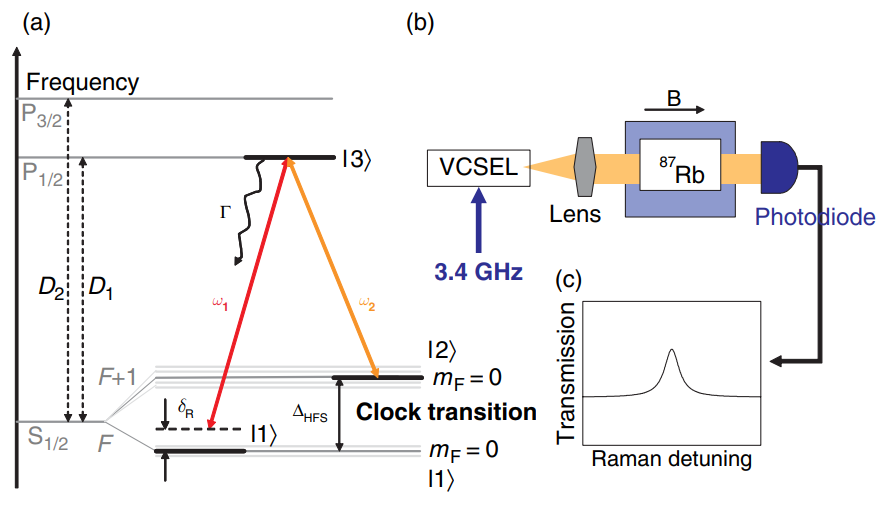
\includegraphics[width=.6\textwidth]{img/atomic_clock_logic}
              \caption{Schematic of the simplified atomic energy level configuration \cite{KNAPPE2008571}}
          \end{figure}

    \item \textbf{Technology Comparison}: Introduce the different types of chip-scale atomic clocks. Compare and contrast the different chip-scale atomic clock technologies in terms of size, power consumption, accuracy, and suitability for various applications.
          \begin{itemize}
              \item Cesium based
              \item Rubidium based
          \end{itemize}
          % \item Fabrication and Manufacturing: Explore the components of chip-scale atomic clocks such as atomic vapor cells, laser systems, and control electronics. Understand the microfabrication techniques used in their manufacturing.
    \item Applications: Consider the diverse applications of chip-scale atomic clocks (aerospace and defense to telecommunications and scientific research)
    \item Challenges and Future Directions: Identify current challenges such as size reduction and power efficiency, and consider future trends like adoption of optical lattice clocks and integration with quantum technologies.
    \item Conclusion: Summarize the key findings of the research and discuss the implications for future advancements and applications of chip-scale atomic clocks.
\end{enumerate}

% In case of time availability, we will also cover the Fabrication and Manufacturing of these devices, understanding the microfabrication techniques used in their manufacturing.

\paragraph{Time schedule}
In general, given a time constraint of 4/5 weeks, the project will be divided as follows (tentative)

\begin{itemize}
    \item Week 1: Introduction + Engineering of Chip-Scale Atomic Clocks
    \item Week 2: Engineering of Chip-Scale Atomic Clocks (possible simulation and results analysis)
    \item Week 3: Technology Comparison + Applications
    \item Week 4: Challenges and Future Directions + Conclusion
    \item Week 5: Final report writing
\end{itemize}

% \section{Results}

\begin{frame}{MSD vs. PCA - Baseline set length ($b$)}

    Here we observe the effect of the baseline set length $b$ on the accuracy of the two methods.

    \begin{figure}[H]
        \centering
        \only<1>{
            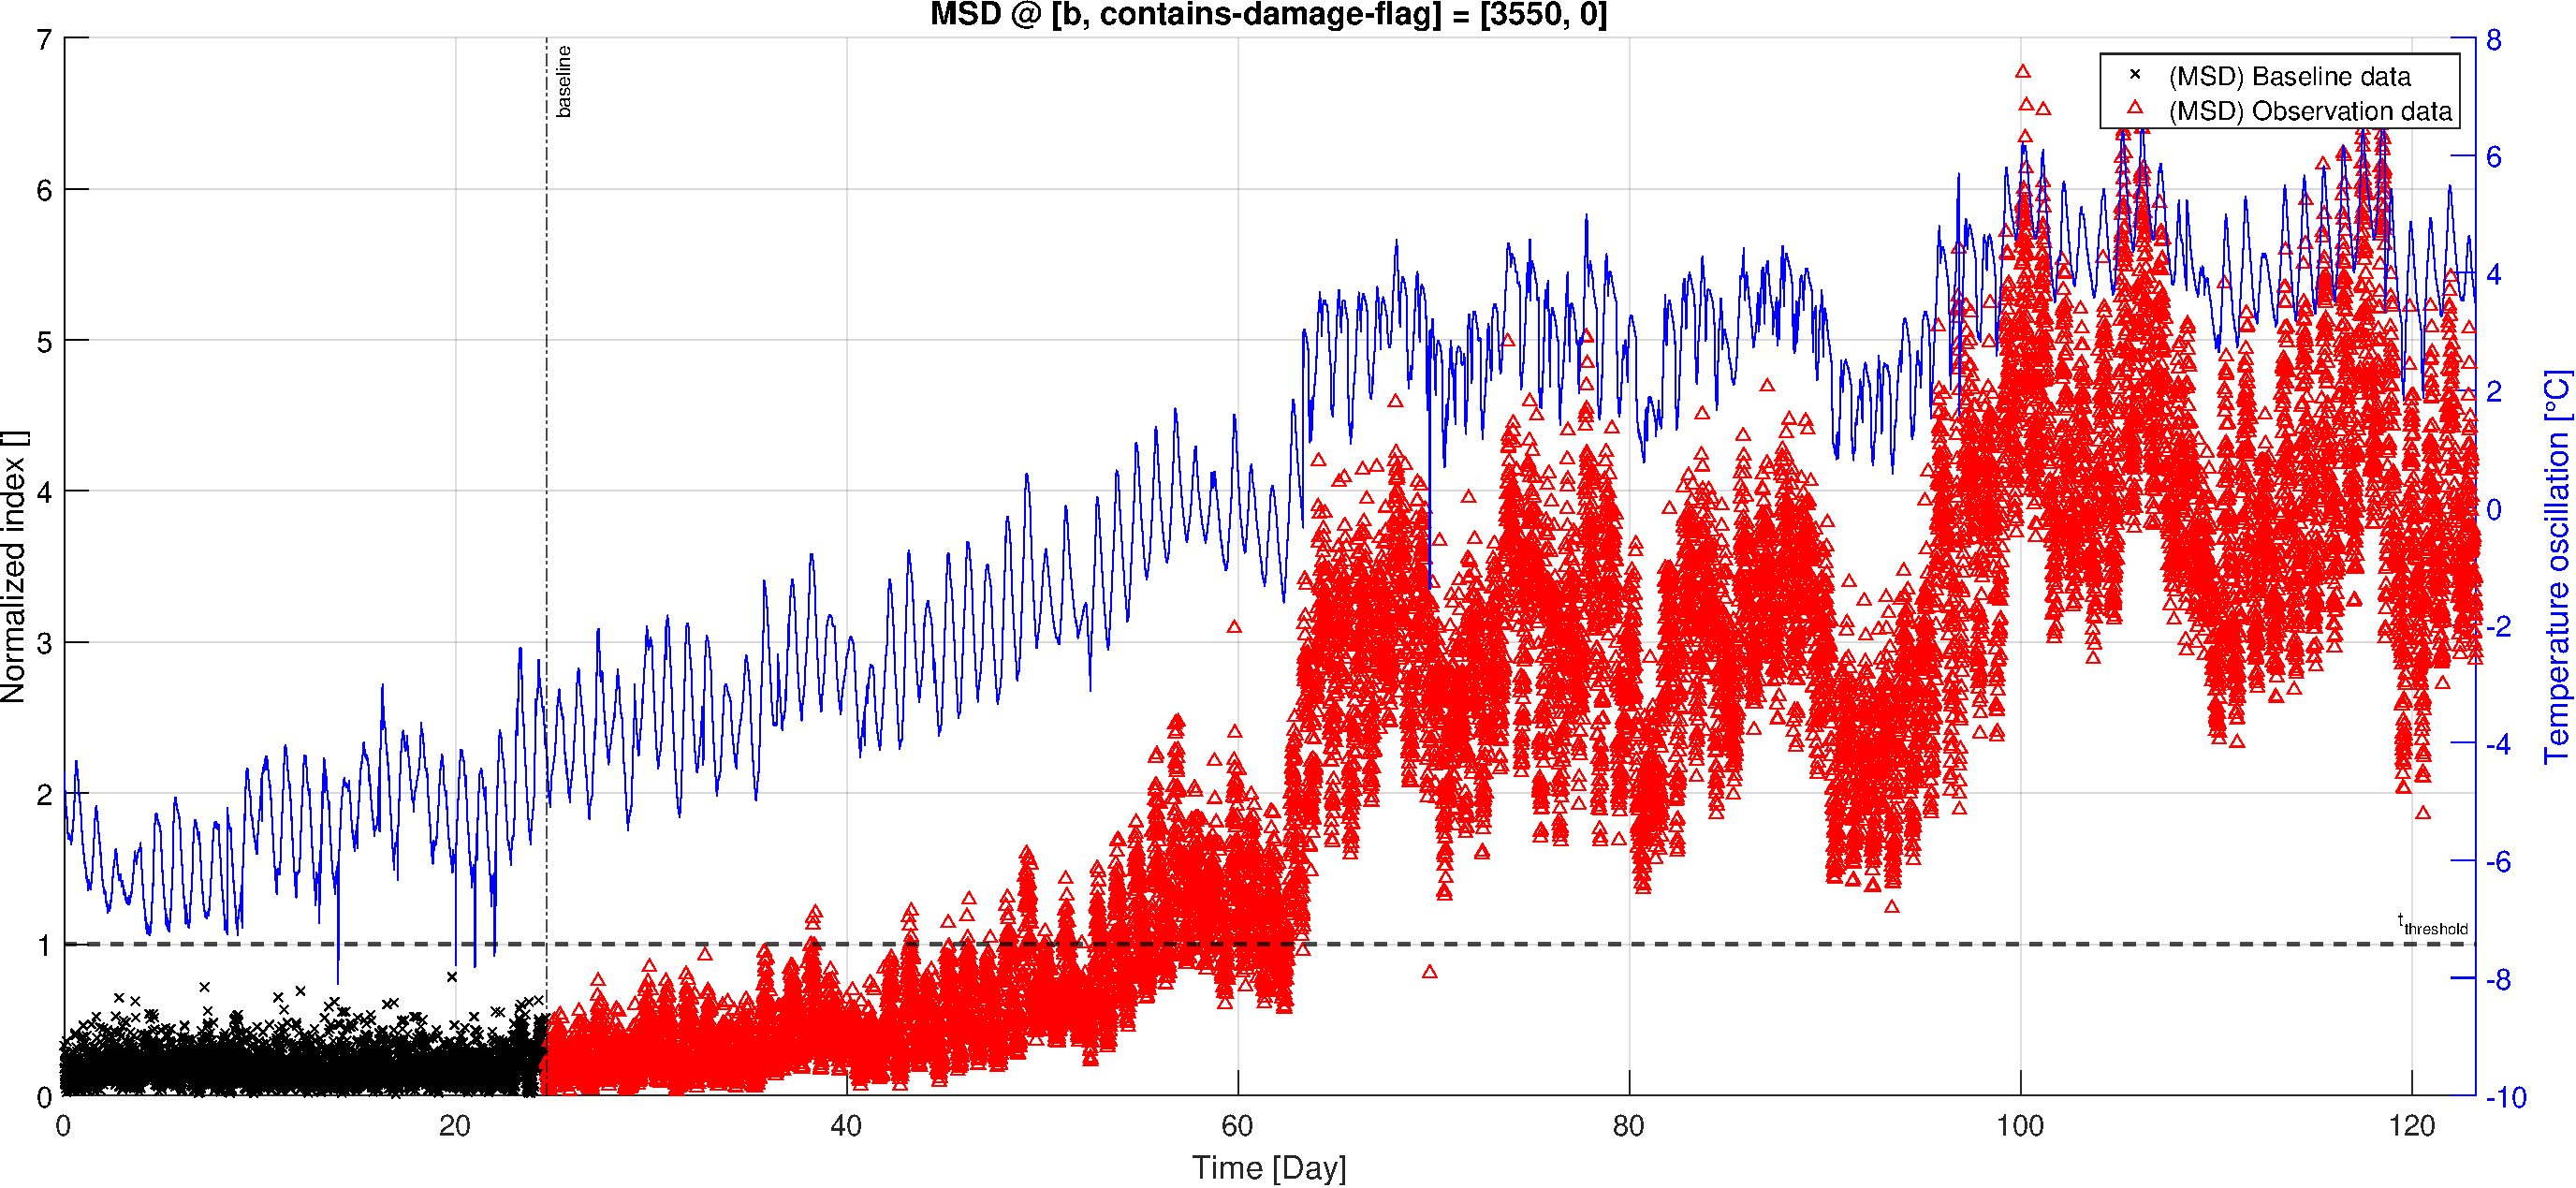
\includegraphics[width=0.9\textwidth]{img/Baseline/MSD_Baseline_3550.pdf}
            \caption{MSD method considering $b = 3550$}
        }
        \only<2>{
            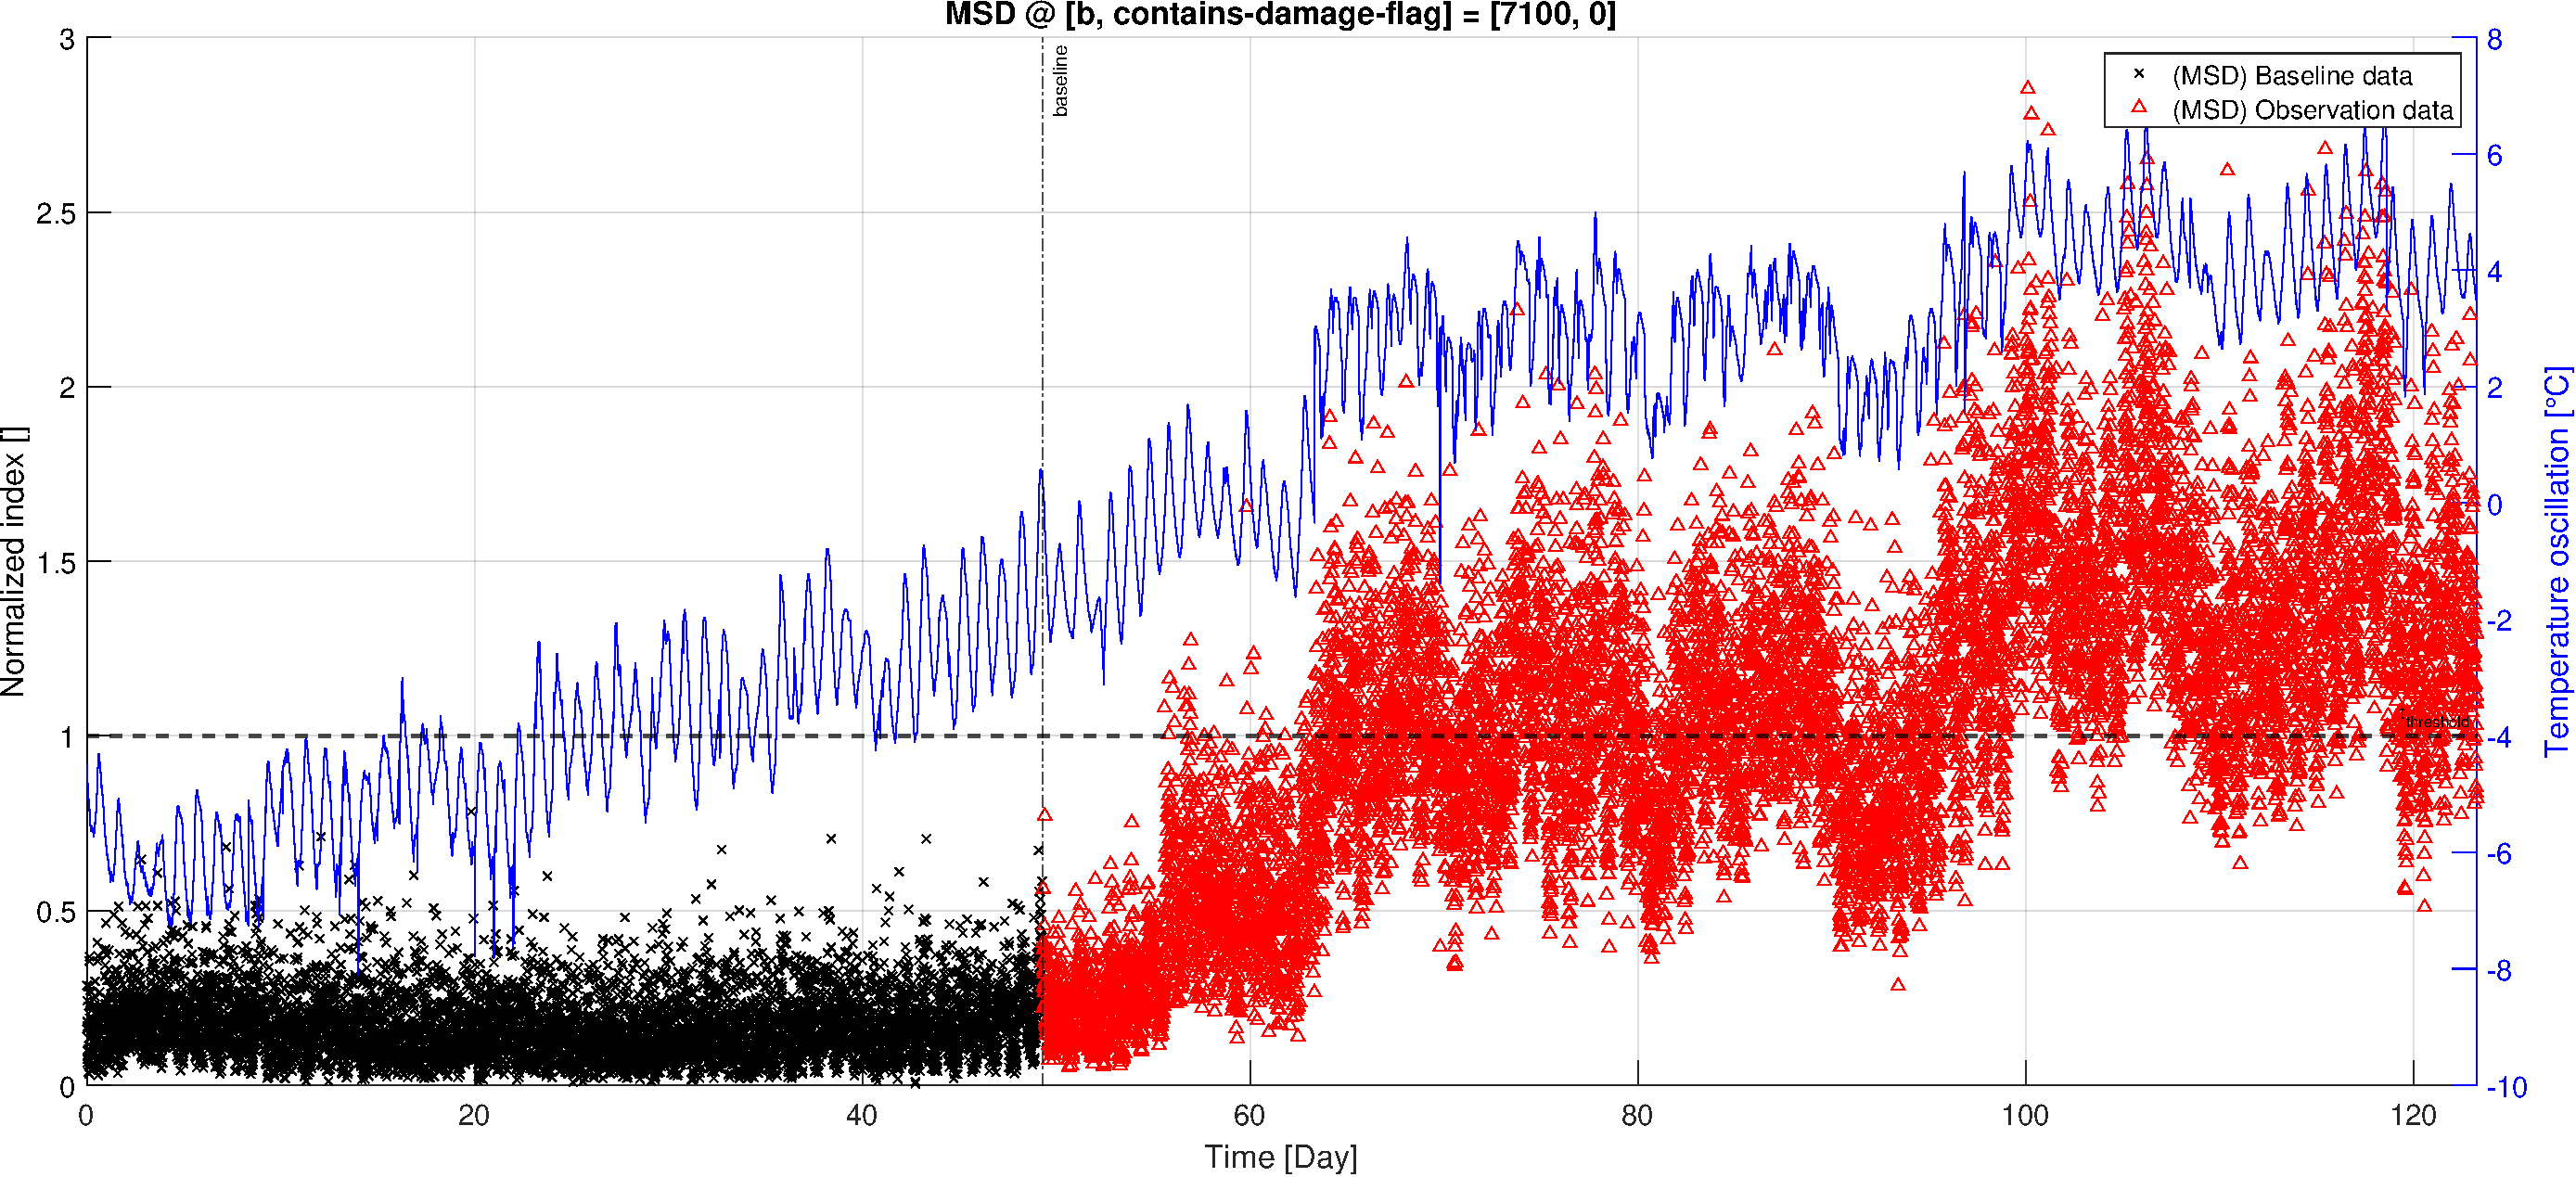
\includegraphics[width=0.9\textwidth]{img/Baseline/MSD_Baseline_7100.pdf}
            \caption{MSD method considering $b = 7100$}
        }
        \only<3>{
            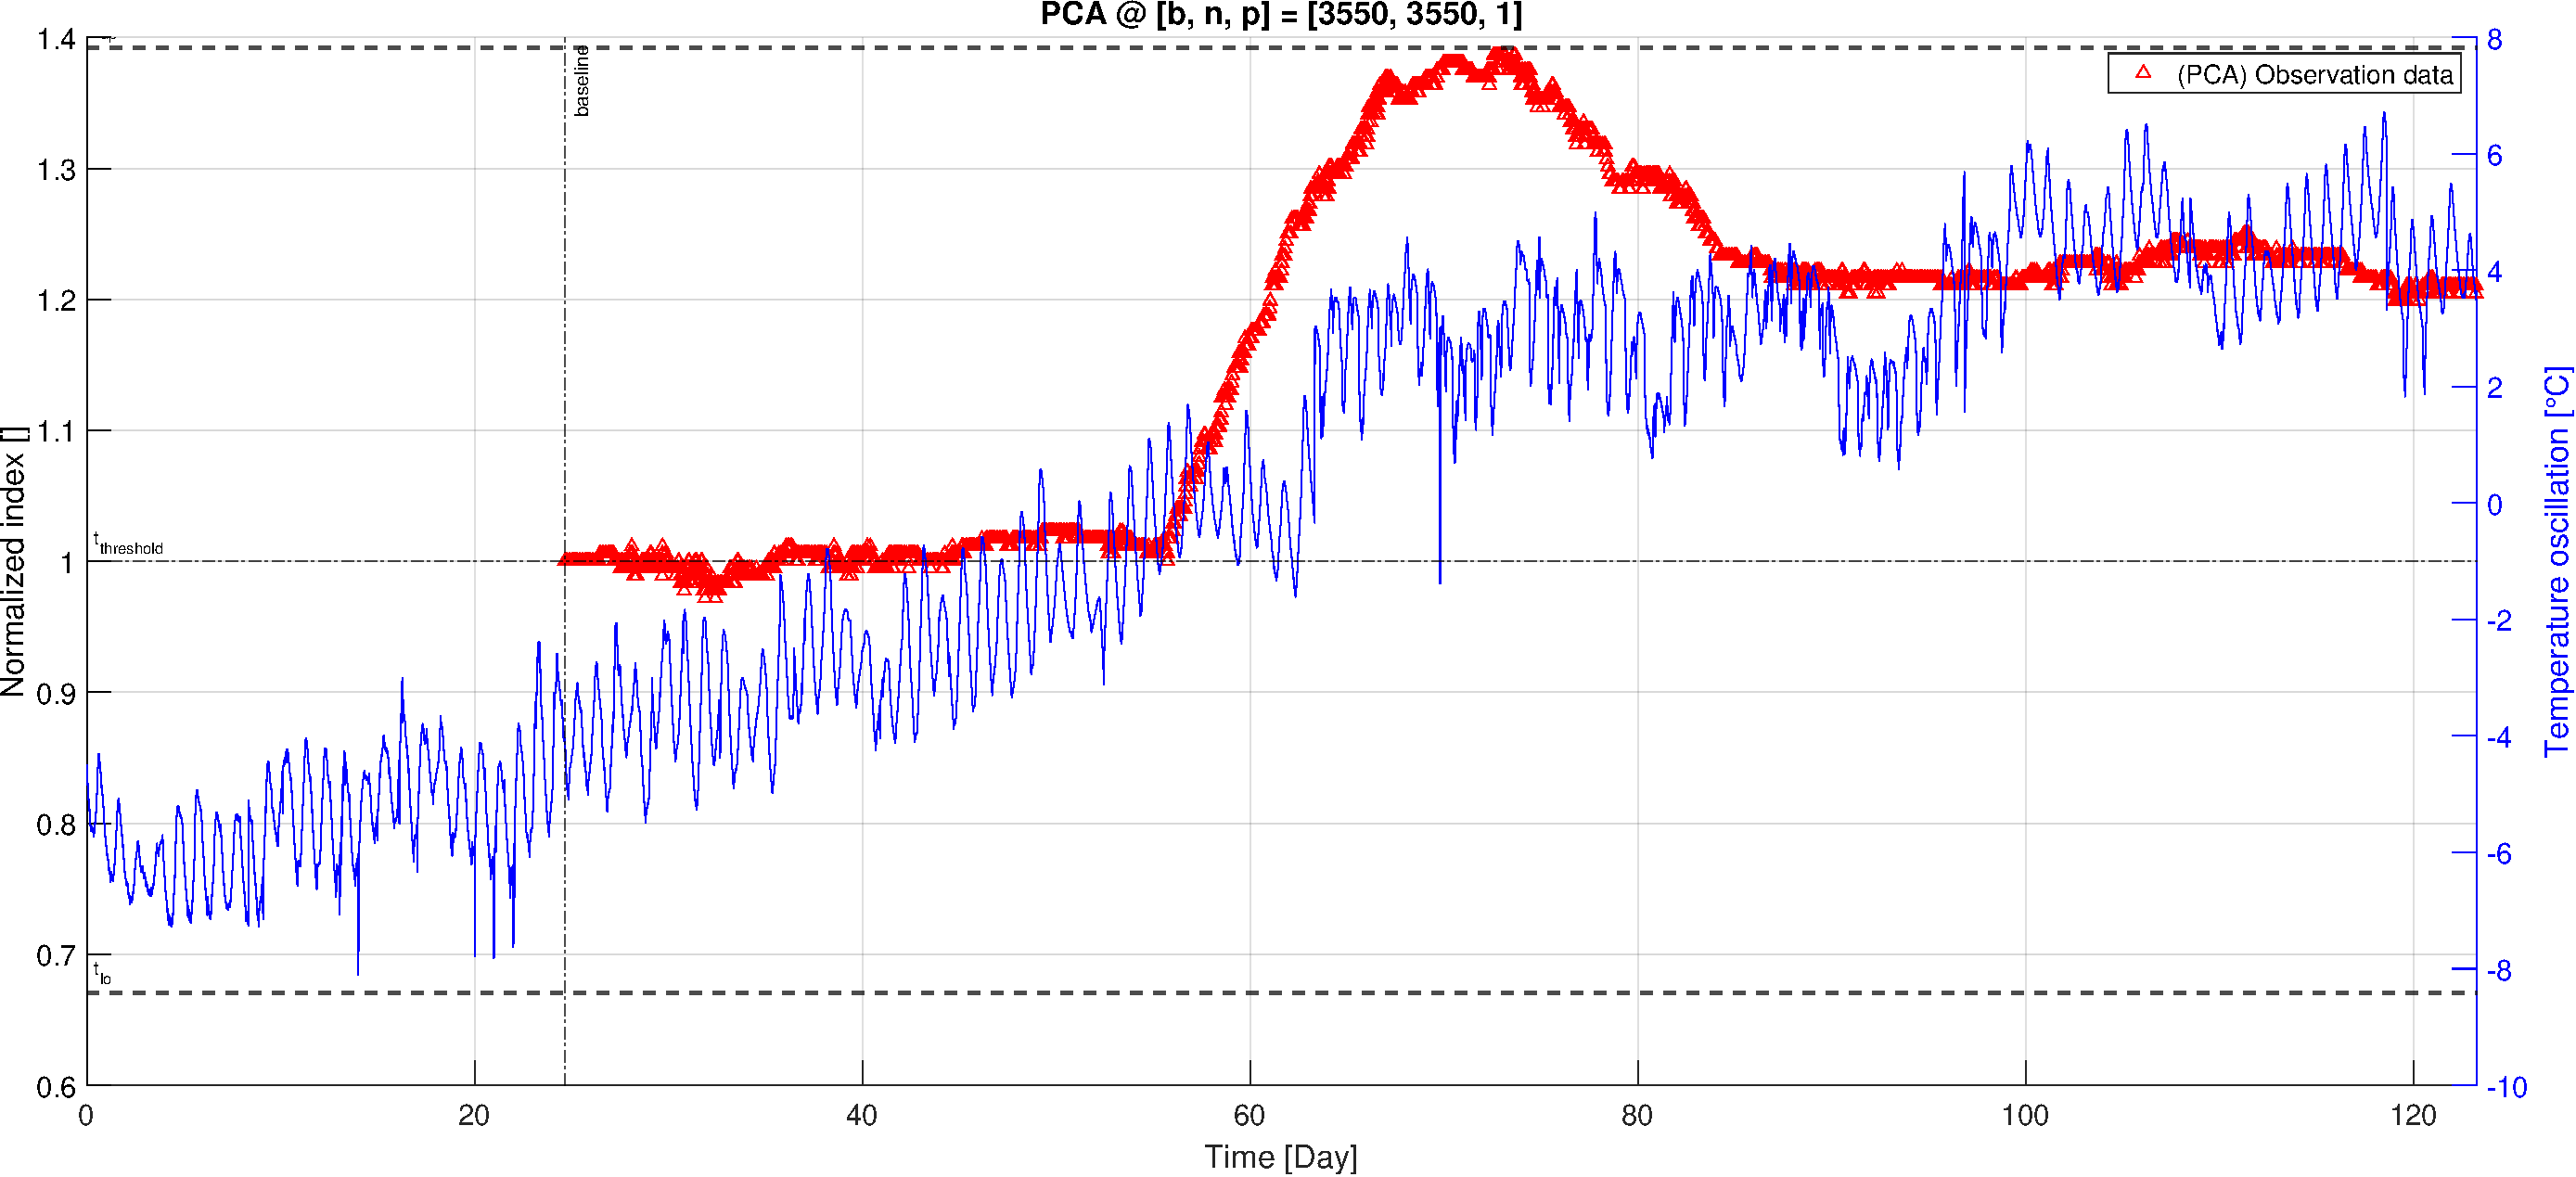
\includegraphics[width=0.9\textwidth]{img/Baseline/PCA_Baseline_3550.pdf}
            \caption{PCA method considering $b = n = 3550$}
        }
        \only<4>{
            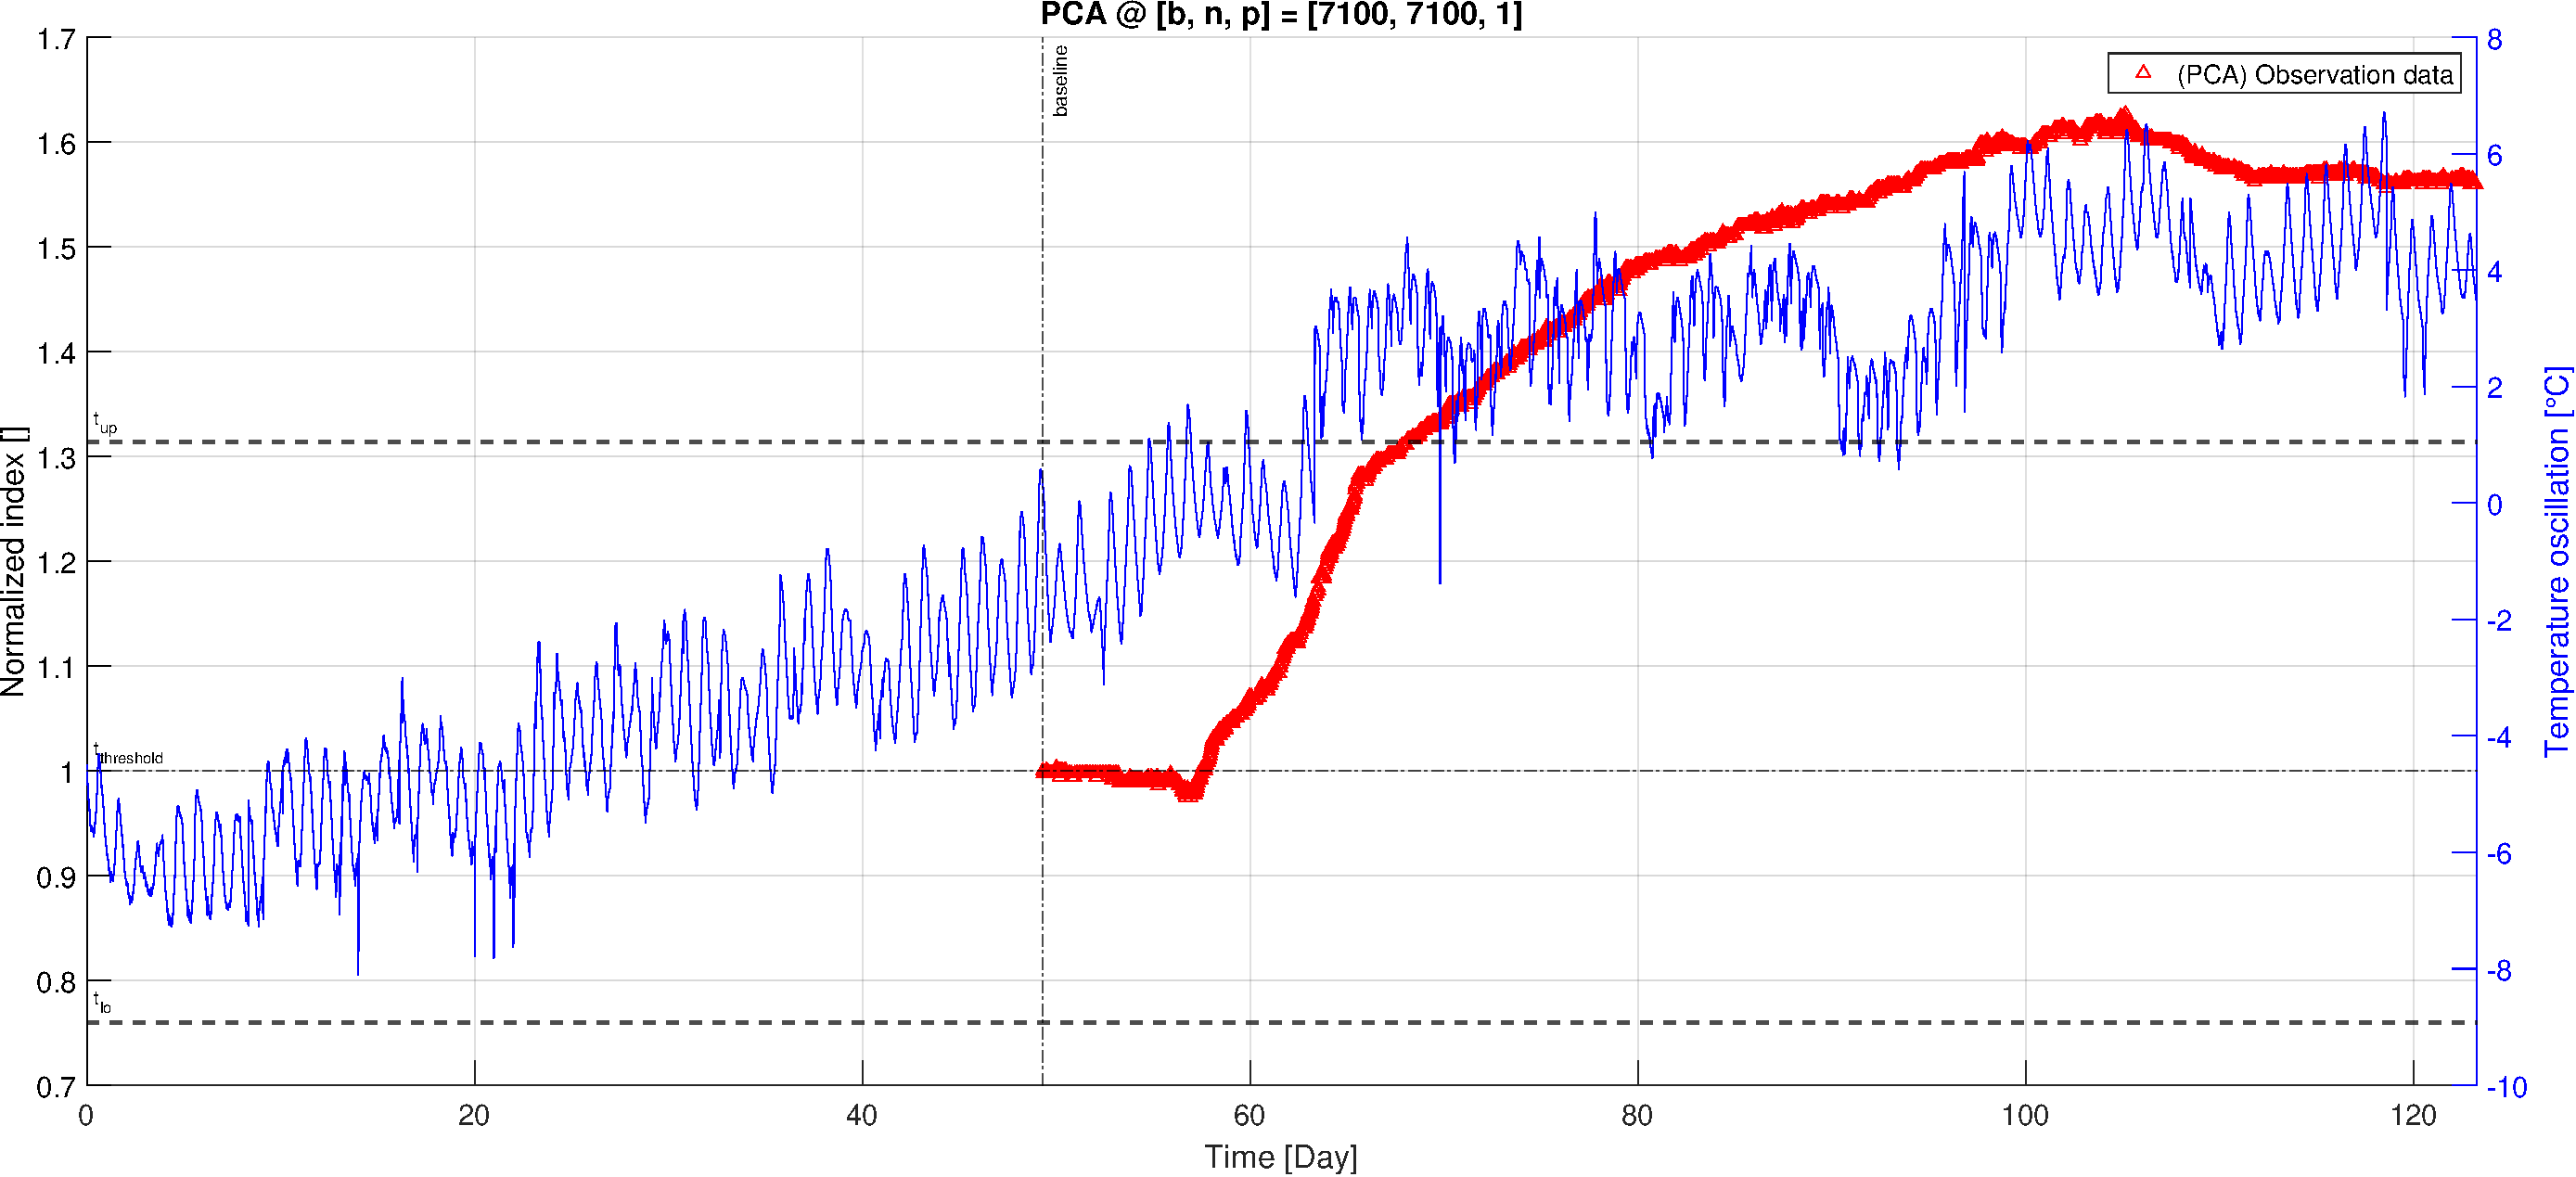
\includegraphics[width=0.9\textwidth]{img/Baseline/PCA_Baseline_7100.pdf}
            \caption{PCA method considering $b = n = 7100$}
        }
    \end{figure}

    \vspace{-9pt}

    \only<1,2>{
        The MSD method is highly sensitive to $b$ and if the baseline set doesn't contain a complete set of environmental conditions, it may lead to false positives/negatives.
    }

    \only<3,4>{
        The PCA method, instead, is able to detect outliers (almost) independently of the baseline set length, thus shorter campaigns can be performed without losing accuracy.
    }

\end{frame}



\begin{frame}{PCA - Observation window length ($n$)}

    A key difference between the MSD and PCA methods is that MSD compute the index for each observation record, while PCA computes the index for a set of records with length $n$.

    \begin{figure}[H]
        \centering
        \only<1>{
            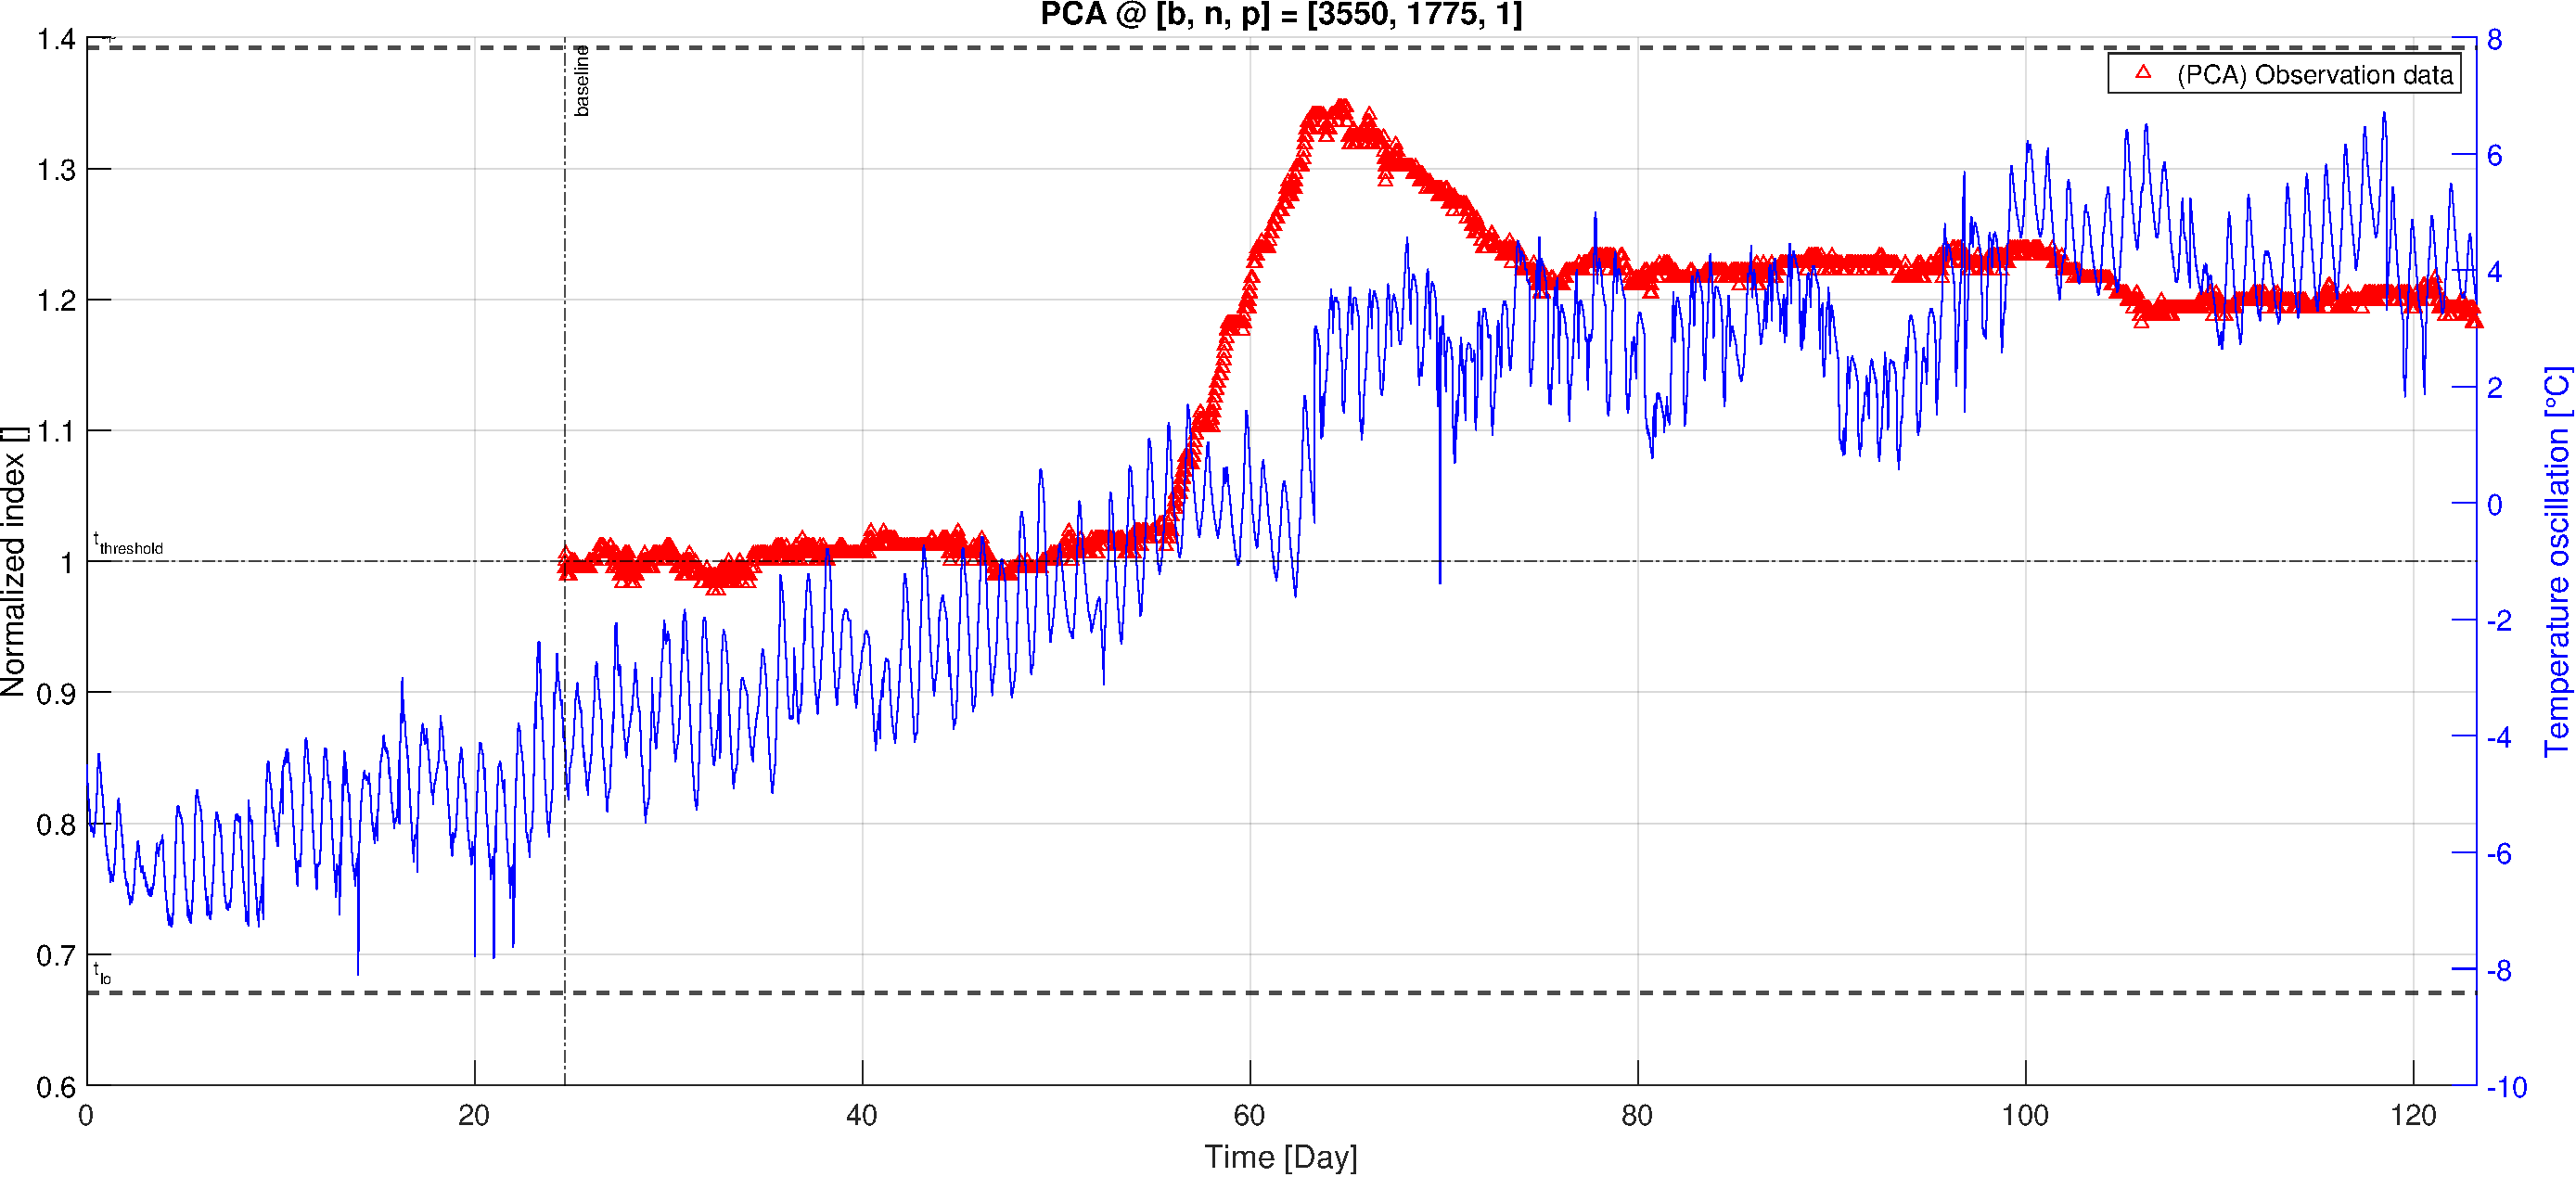
\includegraphics[width=0.9\textwidth]{img/Window/PCA_Window_1775.pdf}
            \caption{PCA method considering $b = 3550$ \& $n = 1775$}
        }
        \only<2>{
            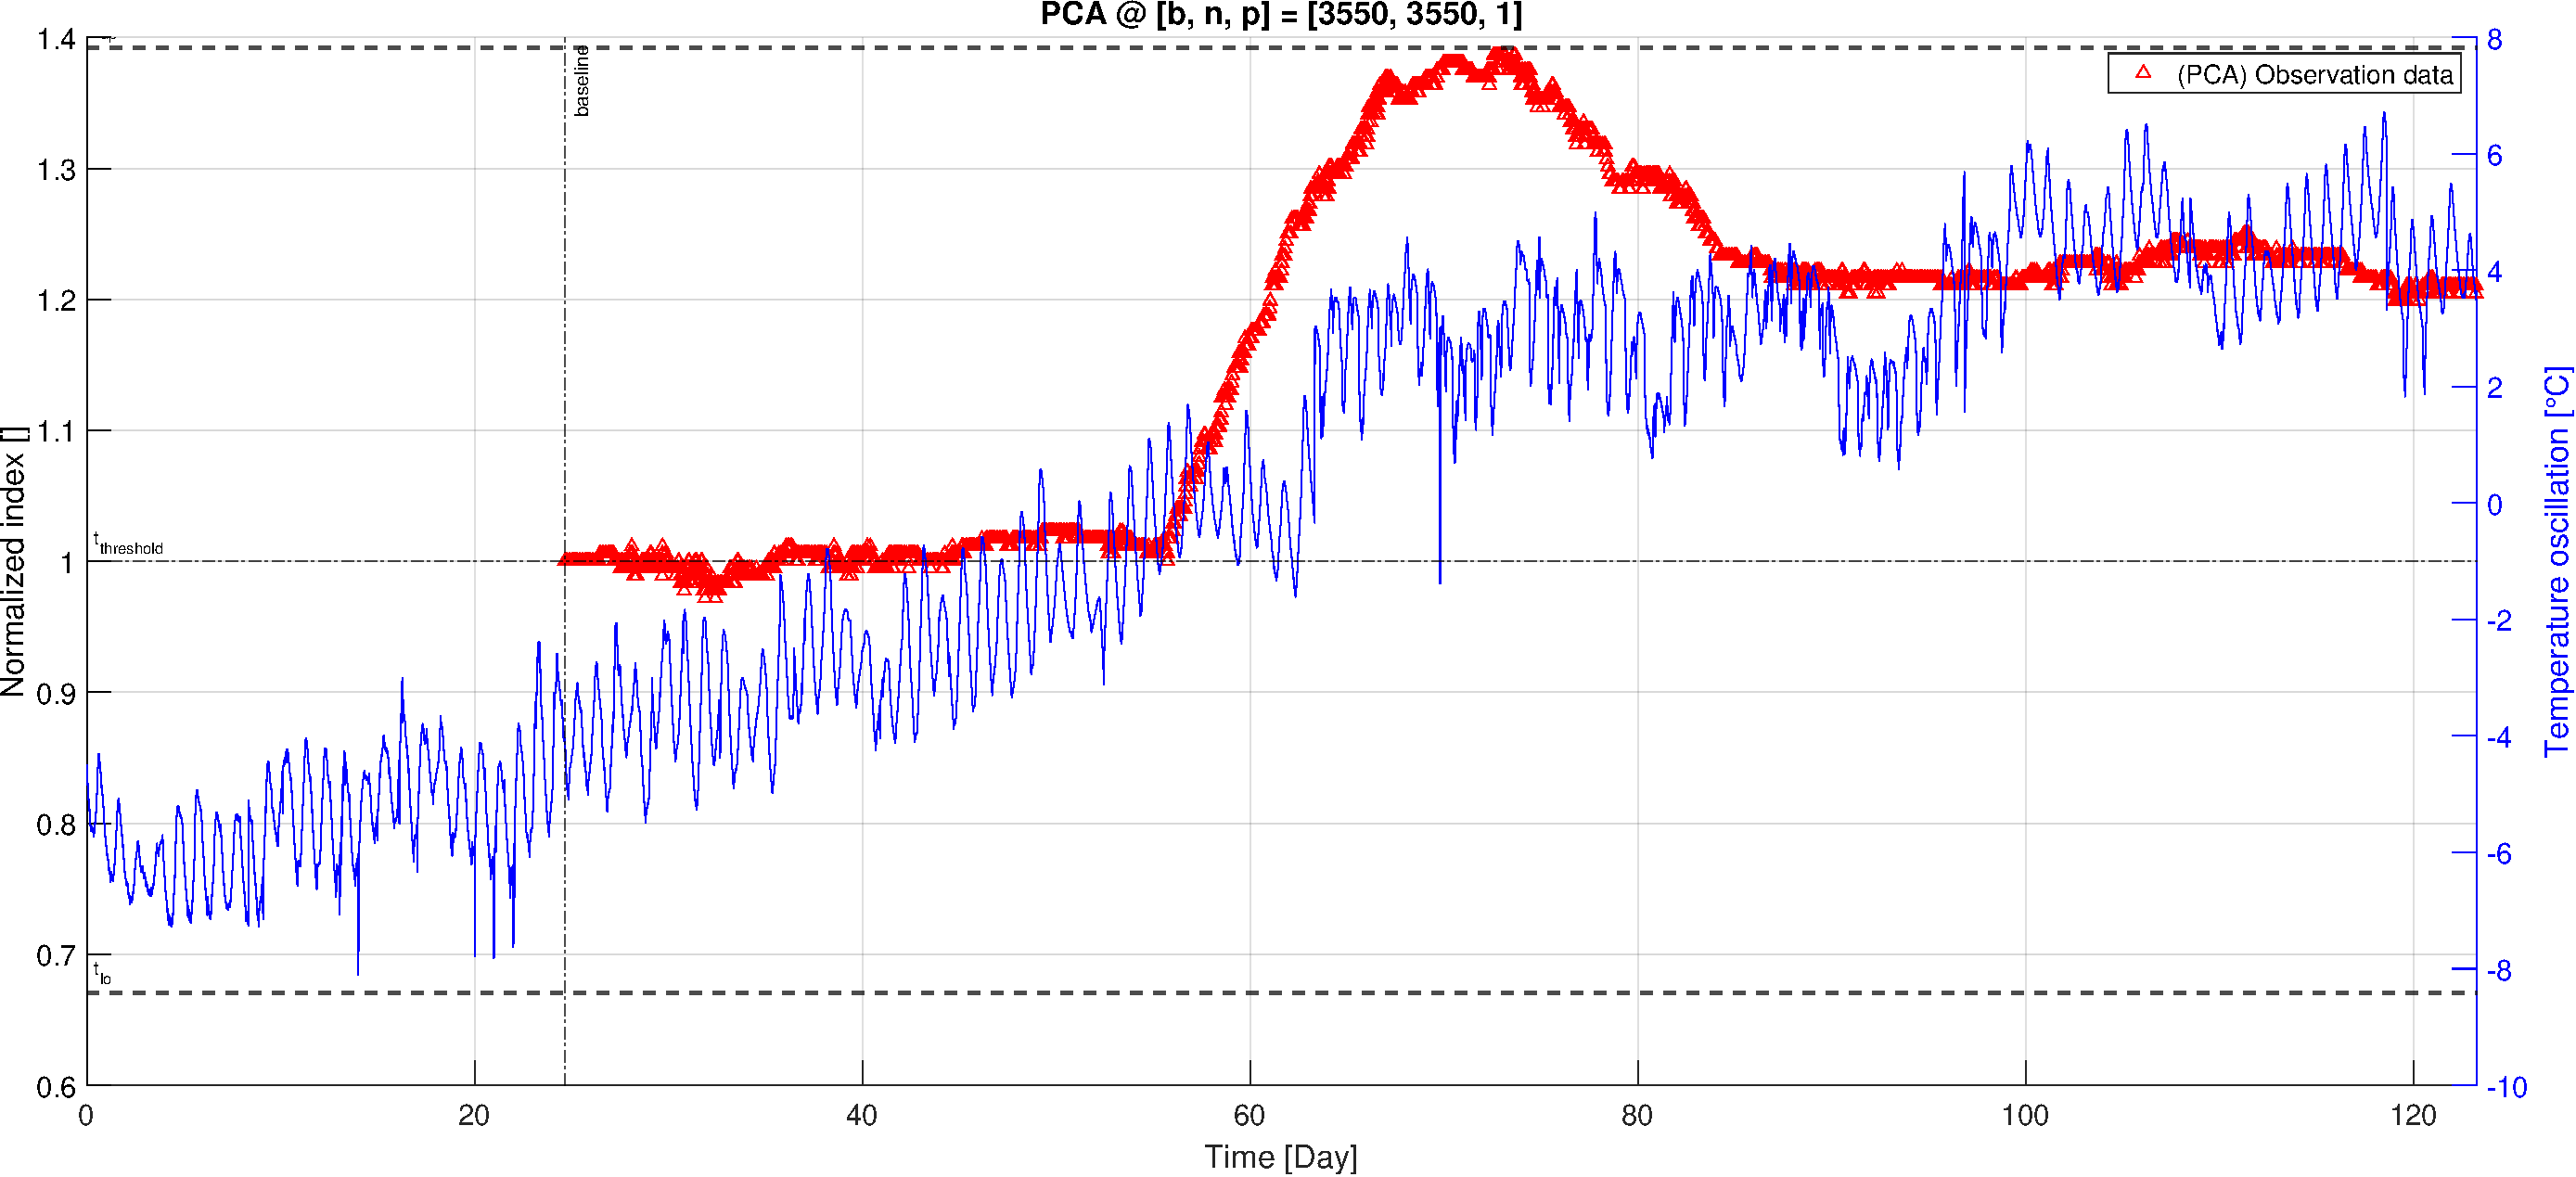
\includegraphics[width=0.9\textwidth]{img/Window/PCA_Window_3550.pdf}
            \caption{PCA method considering $b = 3550$ \& $n = 3550$}
        }
        \only<3>{
            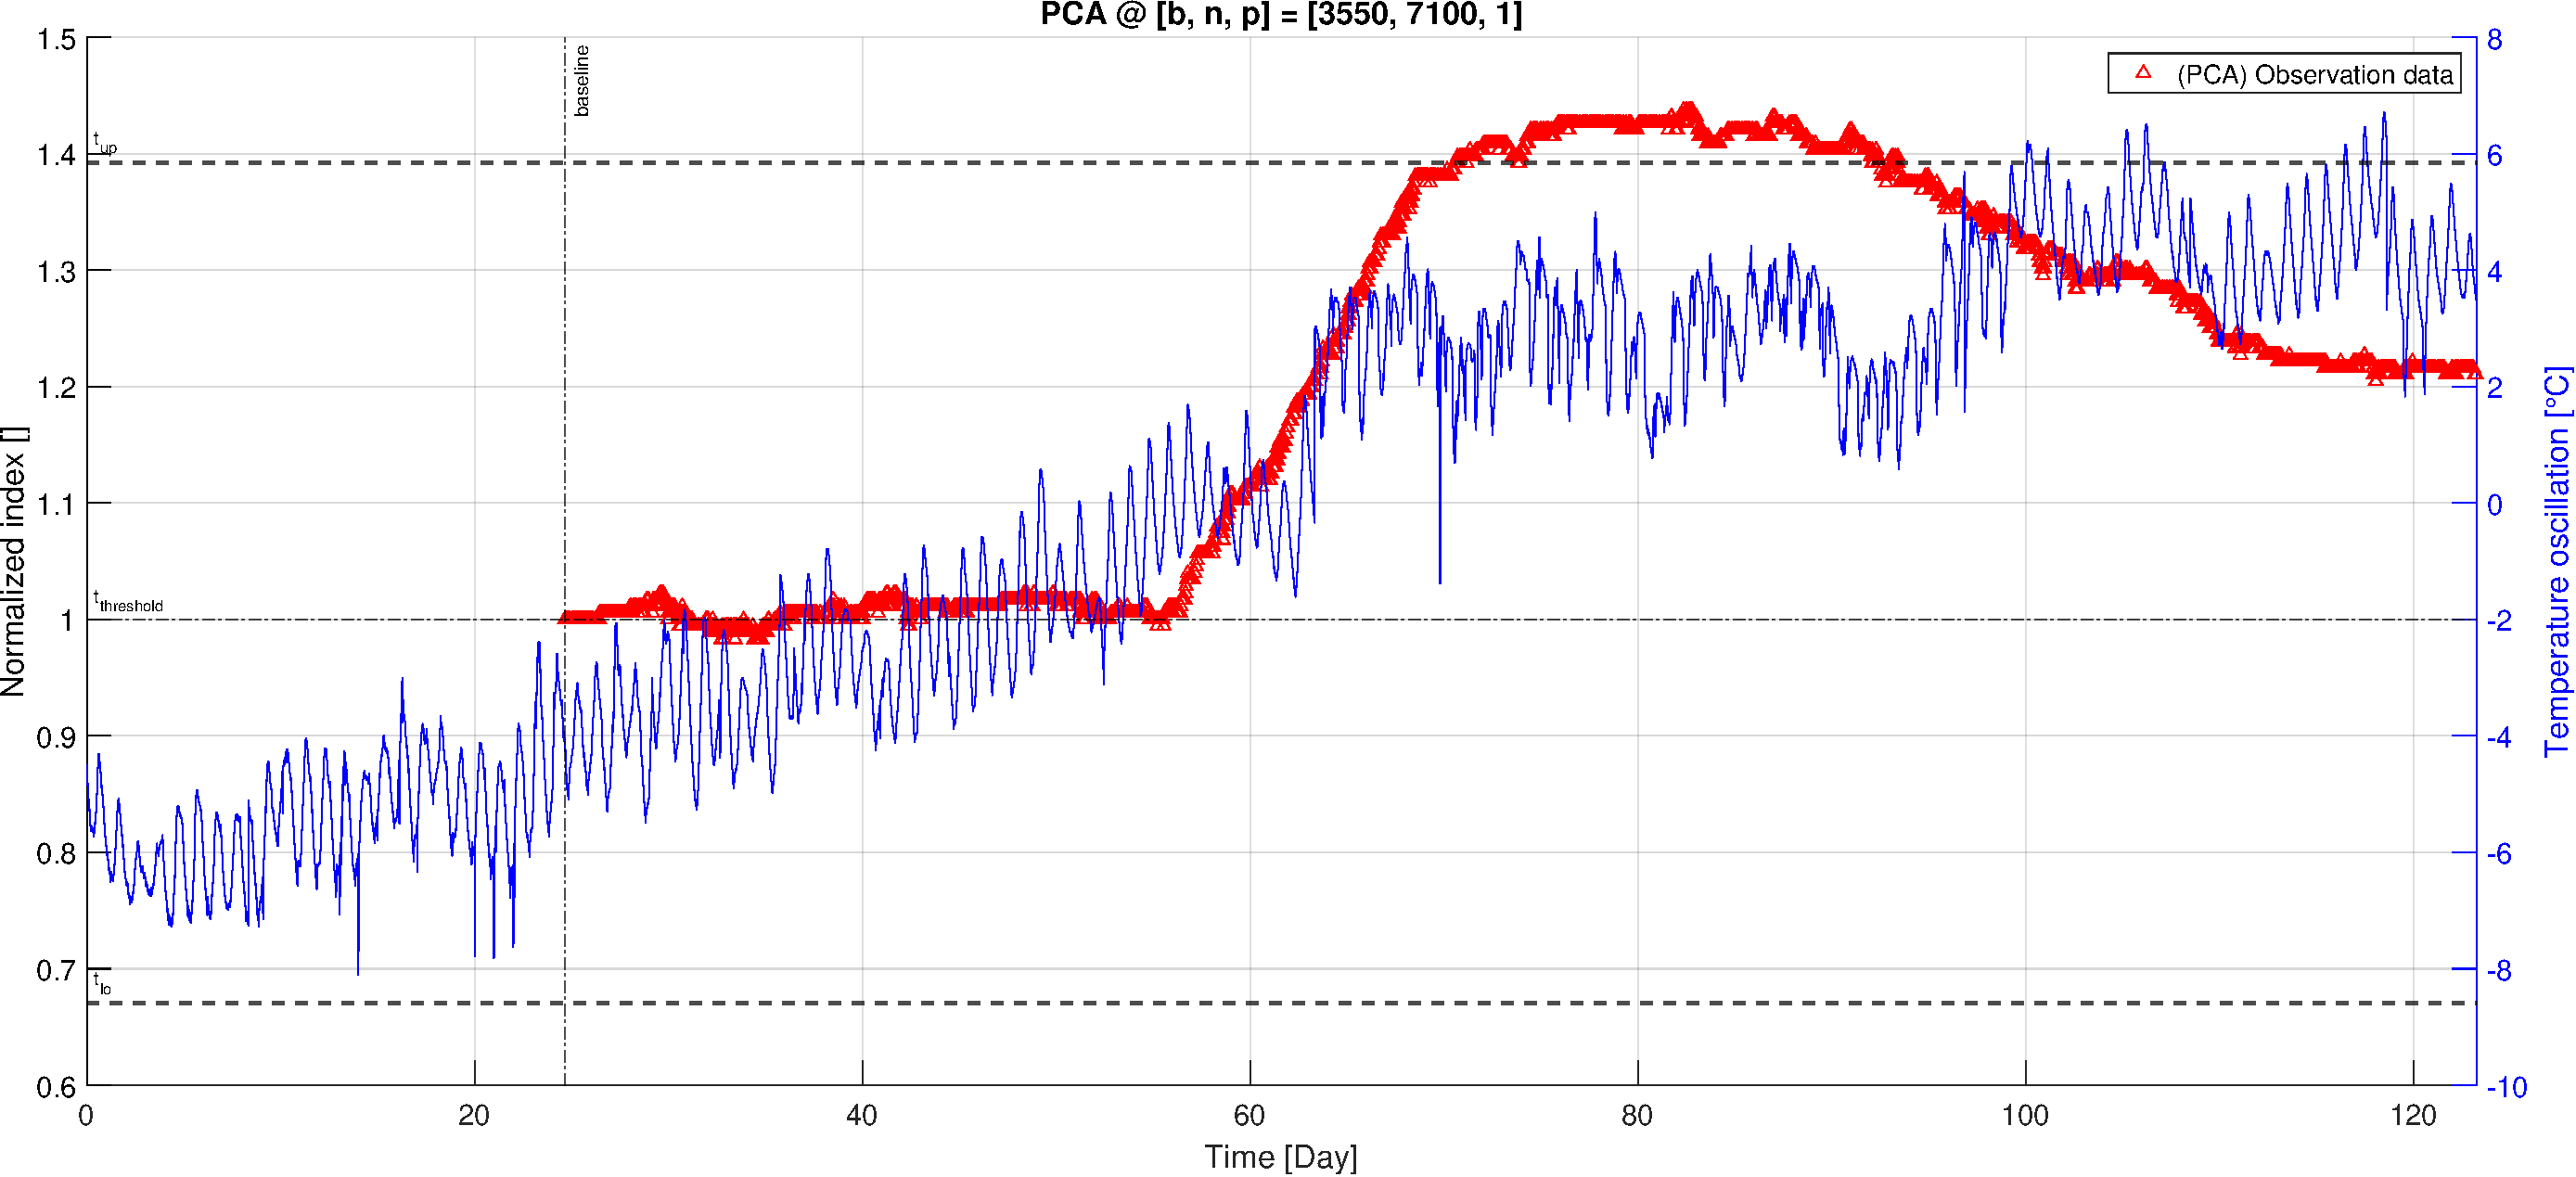
\includegraphics[width=0.9\textwidth]{img/Window/PCA_Window_7100.pdf}
            \caption{PCA method considering $b = 3550$ \& $n = 7100$}
        }
        \only<4>{
            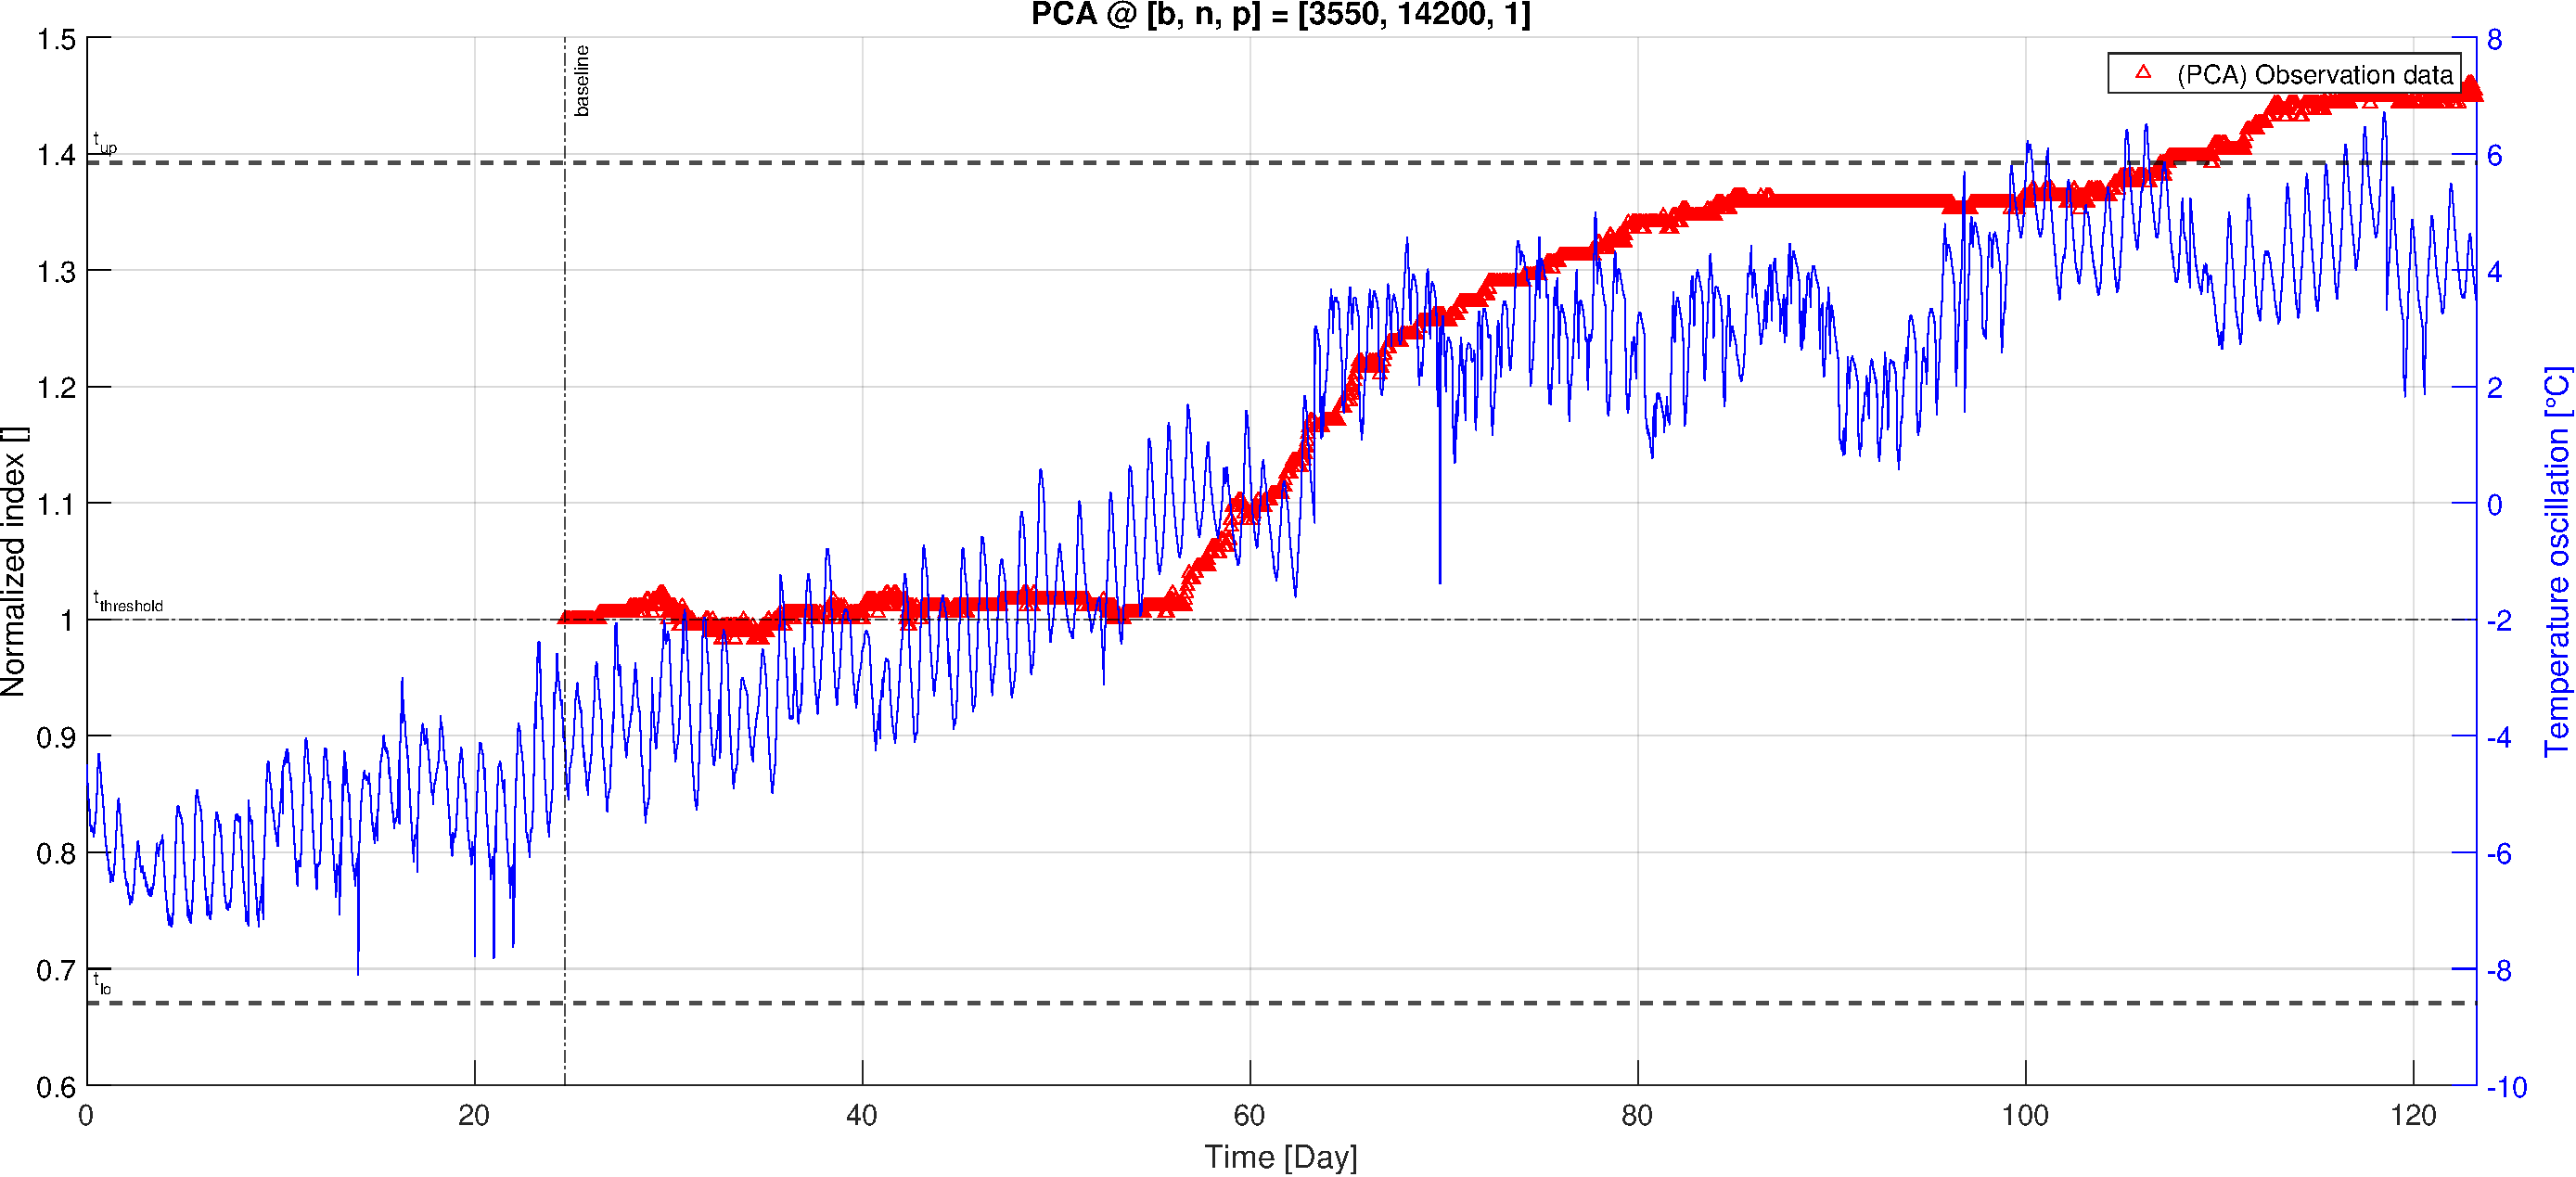
\includegraphics[width=0.9\textwidth]{img/Window/PCA_Window_14200.pdf}
            \caption{PCA method considering $b = 3550$ \& $n = 14200$}
        }
    \end{figure}

    \vspace{-9pt}

    It's clear how $n$ affect the reactivity of the PCA method to detect outliers.
    In particular, the higher $n$, the slower the transient response of the index.

\end{frame}
% \begin{frame}[standout]
    Extra slides
\end{frame}



\begin{frame}{$\mathrm{NO_x}$ Emissions}

    $\mathrm{NO_x}$ emissions are a family of nitrogen oxides that are commonly associated with combustion processes of Ammonia.

    The key factors to reduce the $\mathrm{NO_x}$ emissions are combustion temperature and air-to-fuel ratio.

    \begin{figure}[H]
        \centering
        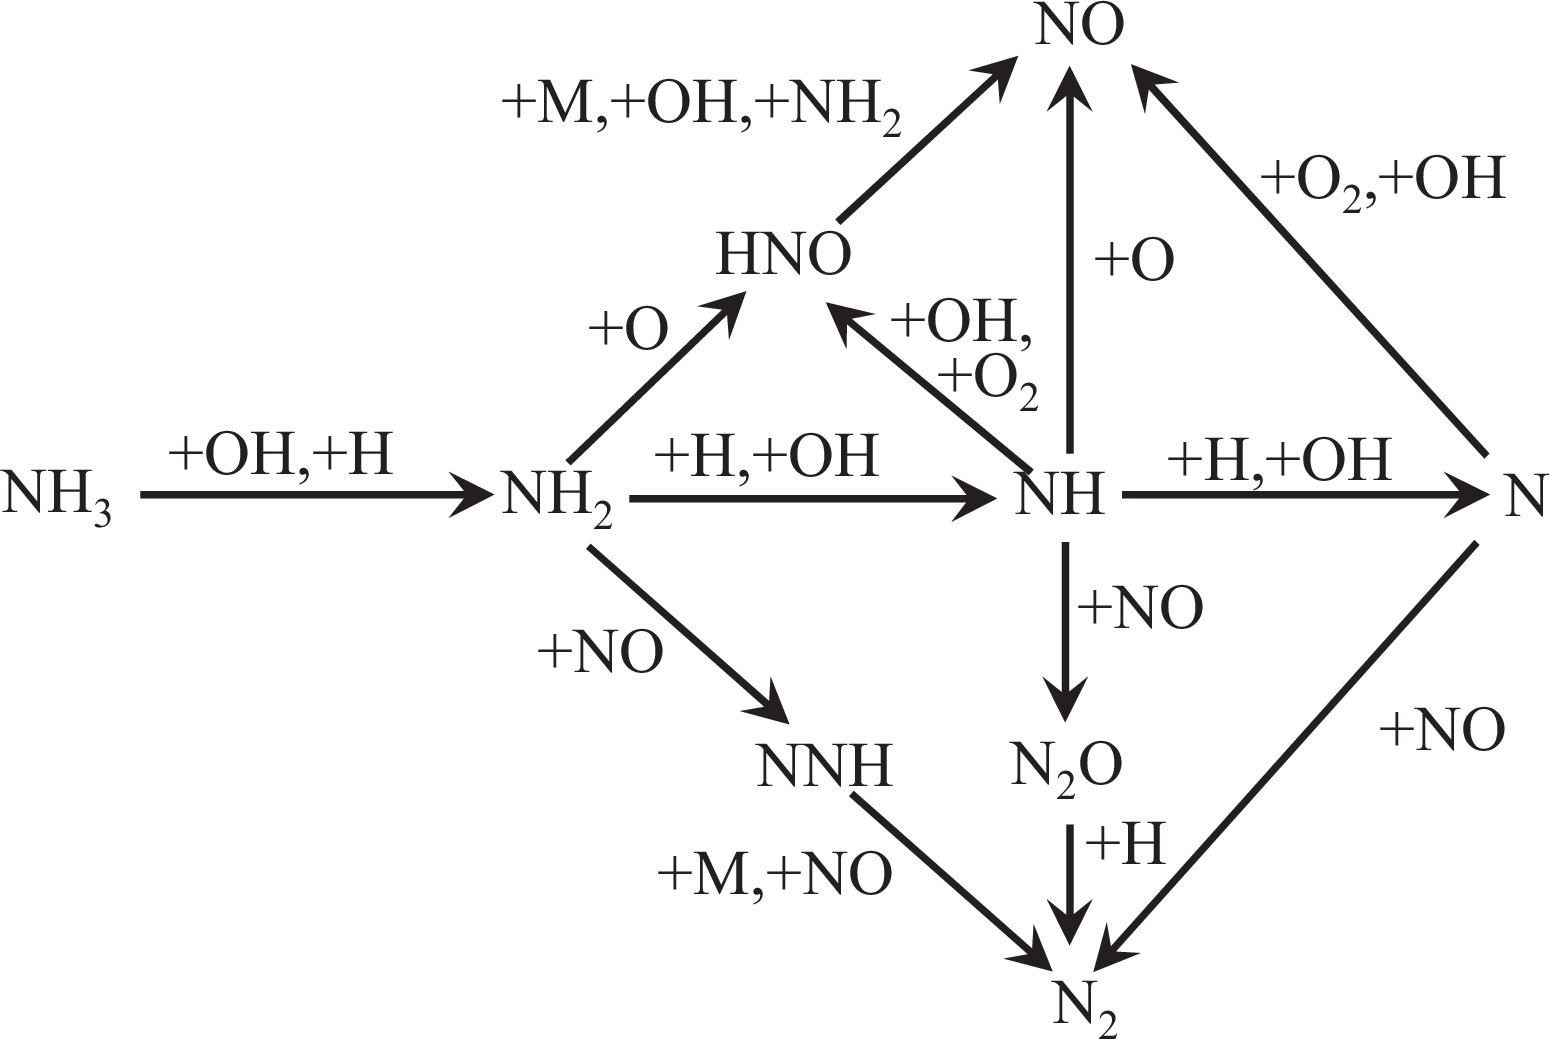
\includegraphics[width=0.6\textwidth]{img/NOx-emission-diagram.jpg}
        \caption{$\mathrm{NH_3}$ oxidation pathway.}
    \end{figure}

\end{frame}



\begin{frame}{Lagrangian vs. Eulerian CFD solver}

    \begin{columns}

        \begin{column}{0.5\textwidth}

            Lagrangian approach consists in \textbf{following droplets during their movement}.

            \begin{figure}[H]
                \centering
                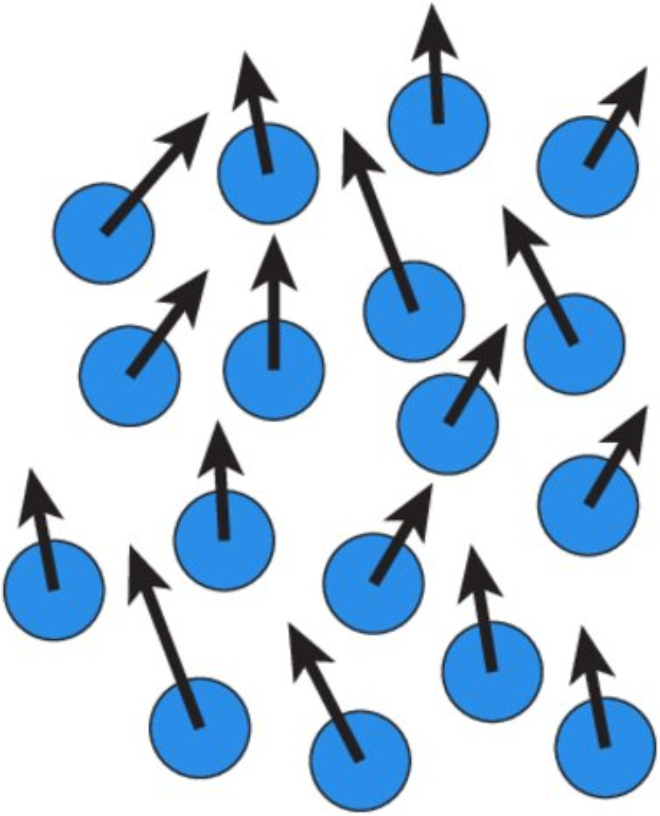
\includegraphics[height=0.5\textheight]{img/extra-lagrangian-approach.png}
                \caption{Lagrangian approach.}
            \end{figure}

        \end{column}

        \begin{column}{0.5\textwidth}

            Eulerian approach consists in \textbf{considering inlet and outlet flux in a given volume}.

            \begin{figure}[H]
                \centering
                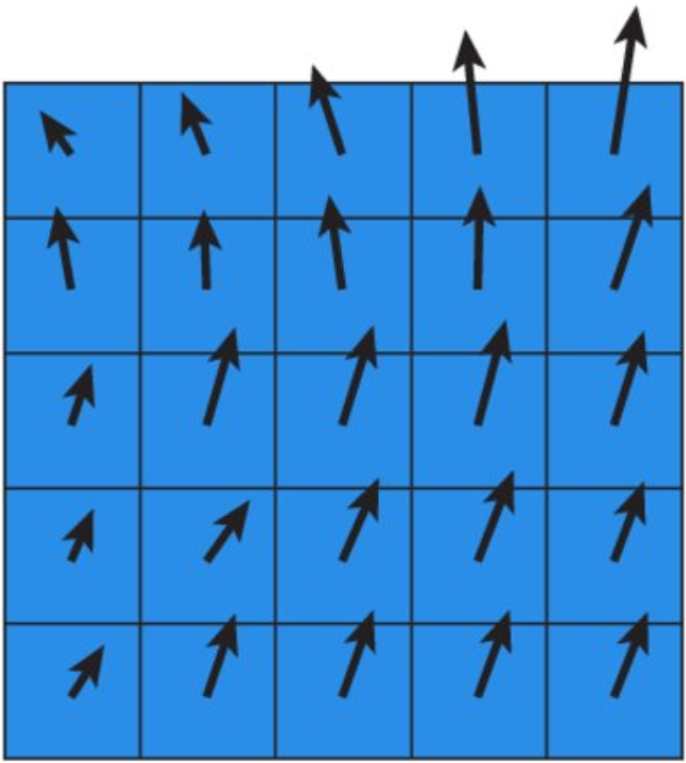
\includegraphics[height=0.5\textheight]{img/extra-eulerian-approach.png}
                \caption{Eulerian approach.}
            \end{figure}

        \end{column}

    \end{columns}

\end{frame}

% \begin{frame}
%     More of the different types of NOx emissions
%     More of the different types of fuel injectors
%     Who uses a suitable replacing combution chamber, what's our target?
% \end{frame}

\appendix

\begin{frame}[allowframebreaks]{References}
    \nocite{*}
    \bibliography{references}
\end{frame}

\begin{frame}[standout]
    Questions?
\end{frame}

\begin{frame}[standout]
    Thank you!
\end{frame}

\end{document}